% ******************************************************************	********************************************
%
% **************************************************************************************************************
\documentclass[ twoside,openright,titlepage,numbers=noenddot,%
				toc=bibliography,toc=listof,%
                footinclude=false,headinclude=false,cleardoublepage=empty,%
				BCOR=5mm,paper=a4,fontsize=11pt
                %,ngerman%
                ]{scrreprt}
%***************************************************************************************************************
% Note: Make all your adjustments in here
%***************************************************************************************************************
% ****************************************************************************************************
% htwsaar-i-mst-config.tex 
% ****************************************************************************************************  
\RequirePackage[utf8]{inputenc}				
 \DeclareUnicodeCharacter{00A0}{~}								
\RequirePackage[T1]{fontenc} 
								
% ****************************************************************************************************
% 1. Personal data and user ad-hoc commands
% ****************************************************************************************************
\newcommand{\myTitle}{Evaluierung lokaler KI-Modelle auf Android für BCI-Anwendungen}
\newcommand{\myDegree}{Bachelor of Science (B.\,Sc.)\xspace}
%\newcommand{\myDegree}{Master of Science (M.\,Sc.)\xspace}
\newcommand{\myDegreeType}{Bachelor\xspace}
%\newcommand{\myDegreeType}{Master\xspace}
\newcommand{\myDegreeCourse}{Praktische Informatik}
%\newcommand{\myDegreeCourse}{Informatik und Web-Engineering}
%\newcommand{\myDegreeCourse}{Kommunikationsinformatik}
%\newcommand{\myDegreeCourse}{Produktionsinformatik}
\newcommand{\myName}{Ahmed Chaabo\xspace}
\newcommand{\myUni}{Hochschule für Technik und Wirtschaft des Saarlandes\xspace}
\newcommand{\myCompany}{SoftwareCenter Musterhausen\xspace}
\newcommand{\myFirstProf}{Prof. Dr. rer. nat. Dr. rer. med. habil. Daniel J.Strauss\xspace}
\newcommand{\mySecondProf}{Prof. Dr.-ing. Klaus Berberich\xspace}
\newcommand{\myLocation}{Saarbrücken\xspace}
\newcommand{\myTime}{Tag.~Monat~Jahr\xspace}
\newcommand{\currentVersion}{Version 2.25, August 2024\xspace} % TODO: ggf. über git Versionsinformationen automatisch bereitstellen und verwenden

% ********************************************************************
% Setup, finetuning, and useful commands
% ********************************************************************
\newcounter{dummy} % necessary for correct hyperlinks (to index, bib, etc.)
% ****************************************************************************************************


% ****************************************************************************************************
% 2. Loading some handy packages
% ****************************************************************************************************
% ******************************************************************** 
% Packages with options that might require adjustments
% ******************************************************************** 
\PassOptionsToPackage{ngerman}{babel}   % change this to your language(s)
 \RequirePackage{babel}					
 \RequirePackage{csquotes}
	
\PassOptionsToPackage{language=auto,style=numeric-comp,backend=biber,bibencoding=ascii,maxbibnames=50}{biblatex} % backend ggf. auf neueres Werkzeug (z.B. biber) anpassen
 \RequirePackage{biblatex}
 %\bibliography{Bibliography}	% alter Befehl
 \addbibresource{Bibliography.bib}

\PassOptionsToPackage{fleqn}{amsmath}		% math environments and more by the AMS 
 \RequirePackage{amsmath}

% ******************************************************************** 
% Setting up the page and margins
% ******************************************************************** 
\usepackage{geometry}
 \geometry{a4paper,left=25mm,right=35mm,top=25mm,bottom=30mm}
% DIESE WERTE SIND NICHT ZU VERÄNDERN -- DO NOT CHANGE THESE VALUES

% ******************************************************************** 
% General useful packages
% ******************************************************************** 
%\usepackage[automark]{scrpage2}
\PassOptionsToPackage{dvipsnames}{xcolor}
	\RequirePackage{xcolor} % [dvipsnames]  
	\definecolor{ingwi}{cmyk}{.9,0,0,0}
\usepackage{textcomp} % fix warning with missing font shapes
\usepackage{scrhack} % fix warnings when using KOMA with listings package          
\usepackage{xspace} % to get the spacing after macros right  
\usepackage{mparhack} % get marginpar right
%\usepackage{fixltx2e} % fixes some LaTeX stuff <-- ist seit 2015 nicht mehr notwendig
\PassOptionsToPackage{printonlyused}{acronym}
	\usepackage{acronym} % nice macros for handling all acronyms in the thesis
%\renewcommand{\bflabel}[1]{{#1}\hfill} % fix the list of acronyms
\usepackage{booktabs}
\usepackage{multirow}
\usepackage{todonotes} %Settings for ToDoNotes
% Eigene Shortcuts fuer laengere Befehle
	\newcommand{\todox}[1]{\todo[inline, size=\small]{#1}}
	%Nummerierte Anmerkungen
	\newcounter{todocounter}
	\renewcommand{\todox}[2][]{\stepcounter{todocounter}\todo[inline, size=\small,caption={\thetodocounter: #2}, #1]{\renewcommand{\baselinestretch}{0.5}\selectfont\thetodocounter: #2\par}}
\usepackage{blindtext}
%\usepackage{footmisc}
% ****************************************************************************************************


% ****************************************************************************************************
% 3. Setup floats: tables, (sub)figures, and captions
% ****************************************************************************************************
\usepackage{tabularx} % better tables
	\setlength{\extrarowheight}{3pt} % increase table row height
%\newcommand{\myfloatalign}{\centering} % to be used with each float for alignment
\usepackage{caption}
\captionsetup{format=hang,font=small}
\usepackage{subfig}
\usepackage{wrapfig}
\usepackage{tikz}
% ****************************************************************************************************


% ****************************************************************************************************
% 6. Setup code listings
% ****************************************************************************************************
\usepackage{listings} 
%\lstset{emph={trueIndex,root},emphstyle=\color{BlueViolet}}%\underbar} % for special keywords
\lstset{language=[LaTeX]Tex,%C++,
    keywordstyle=\color{RoyalBlue},%\bfseries,
    basicstyle=\small\ttfamily,
    %identifierstyle=\color{NavyBlue},
    commentstyle=\color{Green}\ttfamily,
    stringstyle=\rmfamily,
    numbers=none,%left,%
    numberstyle=\scriptsize,%\tiny
    stepnumber=5,
    numbersep=8pt,
    showstringspaces=false,
    breaklines=true,
    frameround=ftff,
    frame=single,
		texcl=true,
    belowcaptionskip=.75\baselineskip
    %frame=L
} 
%Styles für verschiedene Sprachen festlegen, z.B. Java
\lstdefinestyle{Java}{
belowcaptionskip=1\baselineskip,
  breaklines=true,
  xleftmargin=\parindent,
  language=Java,
	texcl=true,
  showstringspaces=false,
  basicstyle=\footnotesize\ttfamily,
  keywordstyle=\bfseries\color{green!40!black},
  commentstyle=\itshape\color{purple!40!black},
  identifierstyle=\color{blue},
  stringstyle=\color{orange}}

% Farben fuer den Quellcode-Stil (an gaengiger IDE-Optik orientiert)
\definecolor{lstframe}{gray}{0.6}         % grauer Rahmen
\definecolor{lstbg}{gray}{0.985}          % sehr heller Hintergrund
\definecolor{lstkw}{RGB}{20,40,150}       % Schluesselwoerter: dunkelblau
\definecolor{lsttype}{RGB}{0,128,128}     % Typen/Klassen: teal
\definecolor{lstconst}{RGB}{130,50,150}   % Konstanten: violett
\definecolor{lstnum}{RGB}{160,90,0}       % Zahlen: orange-braun
\definecolor{lstcomment}{gray}{0.5}       % Kommentare: grau
\definecolor{lststring}{RGB}{0,120,80}    % Strings: gruen

% Eigener Stil fuer Quellcode-Listings: Padding, kein Umbruch, nicht ueber Seiten splitten
\lstdefinestyle{code}{
  language=Java,
  basicstyle=\footnotesize\ttfamily\color{black!88},
  keywordstyle=\bfseries\color{lstkw},
  keywordstyle=[2]\color{lsttype},        % Typen/Klassen
  keywordstyle=[3]\color{lstconst},        % Konstanten
  commentstyle=\itshape\color{lstcomment},
  stringstyle=\color{lststring},
  showstringspaces=false,
  texcl=false,               % Kommentare literal (kein LaTeX) -> % und -> sind unproblematisch
  breaklines=false,          % kein Zeilenumbruch
  % zusaetzliche Wortklassen (2 = Typen, 3 = Konstanten)
  morekeywords=[2]{String,List,ArrayList,Arrays,SampleEntity,SessionFeatures,%
    Segment,FrequencyBand,Check,StringBuilder,Context,LlmInference,%
    LlmInferenceOptions,LlmEngine,StreamCallback,CountDownLatch,Metrics,%
    Runnable,Thread,View,Debug,MemoryInfo,BatteryManager,File,FileWriter,%
    EegFeatureExtractor,FeatureFormatter,PromptBuilder},
  morekeywords=[3]{NUM_BANDS,CHANNELS,SAMPLE_RATE,SEGMENT_COUNT,%
    MAX_INVALID_RATIO,OK,TOO_SHORT,TOO_MANY_INVALID},
  % Zahlen einfaerben
  literate=%
    {0}{{\color{lstnum}0}}1 {1}{{\color{lstnum}1}}1 {2}{{\color{lstnum}2}}1
    {3}{{\color{lstnum}3}}1 {4}{{\color{lstnum}4}}1 {5}{{\color{lstnum}5}}1
    {6}{{\color{lstnum}6}}1 {7}{{\color{lstnum}7}}1 {8}{{\color{lstnum}8}}1
    {9}{{\color{lstnum}9}}1,
  frame=single,
  rulecolor=\color{lstframe}, % grauer Rahmen statt schwarz
  backgroundcolor=\color{lstbg},
  framesep=8pt,              % Innenabstand: Rahmen -> Code (Padding)
  xleftmargin=14pt,          % Abstand links
  xrightmargin=14pt,         % Abstand rechts
  aboveskip=1.2\baselineskip,
  belowskip=1.2\baselineskip,
  belowcaptionskip=1\baselineskip,
  captionpos=b,
}
% ****************************************************************************************************


% ****************************************************************************************************
% 6. PDFLaTeX, hyperreferences and citation backreferences
% ****************************************************************************************************
% ********************************************************************
% Using PDFLaTeX
% ********************************************************************
\usepackage{xurl}  % better handling of long URLs / hyphenation
\PassOptionsToPackage{pdftex,hyperfootnotes=false,pdfpagelabels}{hyperref}
	\usepackage{hyperref}  % backref linktocpage pagebackref
\pdfcompresslevel=9
\pdfadjustspacing=1 
\PassOptionsToPackage{pdftex}{graphicx}
	\usepackage{graphicx} 
    

% ********************************************************************
% Hyperreferences
% ********************************************************************
\hypersetup{%
    %draft,	% = no hyperlinking at all (useful in b/w printouts)
    pdfstartpage=1, pdfstartview=Fit,%
	colorlinks=true, linktocpage=true,
	%urlcolor=Black, linkcolor=Black, citecolor=Black, %pagecolor=Black,%
	%urlcolor=brown, linkcolor=RoyalBlue, citecolor=green, %pagecolor=RoyalBlue,%
    % uncomment the following line if you want to have black links (e.g., for printing)
    colorlinks=false, pdfborder={0 0 0},
    breaklinks=true, pdfpagemode=UseNone, pageanchor=true, pdfpagemode=UseOutlines,%
    plainpages=false, bookmarksnumbered, bookmarksopen=true, bookmarksopenlevel=1,%
    hypertexnames=true, pdfhighlight=/O,%nesting=true,%frenchlinks,%
    pdftitle={\myTitle},%
    pdfauthor={\textcopyright\ \myName, \myUni},%
    pdfsubject={},%
    pdfkeywords={},%
    pdfcreator={pdfLaTeX},%
    pdfproducer={LaTeX with hyperref}%
}   

% ********************************************************************
% Setup autoreferences
% ********************************************************************
% There are some issues regarding autorefnames
% http://www.ureader.de/msg/136221647.aspx
% http://www.tex.ac.uk/cgi-bin/texfaq2html?label=latexwords
% you have to redefine the makros for the 
% language you use, e.g., american, ngerman
% (as chosen when loading babel/AtBeginDocument)
% ********************************************************************
\makeatletter
\@ifpackageloaded{babel}%
    {%
       \addto\extrasamerican{%
					\renewcommand*{\figureautorefname}{Figure}%
					\renewcommand*{\tableautorefname}{Table}%
					\renewcommand*{\partautorefname}{Part}%
					\renewcommand*{\chapterautorefname}{Chapter}%
					\renewcommand*{\sectionautorefname}{Section}%
					\renewcommand*{\subsectionautorefname}{Section}%
					\renewcommand*{\subsubsectionautorefname}{Section}% 	
				}%
       \addto\extrasngerman{% 
					\renewcommand*{\chapterautorefname}{Kapitel}%
					\renewcommand*{\sectionautorefname}{Abschnitt}%
					\renewcommand*{\subsectionautorefname}{Abschnitt}%
					\renewcommand*{\subsubsectionautorefname}{Abschnitt}% 
					\renewcommand*{\paragraphautorefname}{Absatz}%
					\renewcommand*{\subparagraphautorefname}{Absatz}%
					\renewcommand*{\footnoteautorefname}{Fußnote}%
					\renewcommand*{\FancyVerbLineautorefname}{Zeile}%
					\renewcommand*{\theoremautorefname}{Theorem}%
					\renewcommand*{\appendixautorefname}{Anhang}%
					\renewcommand*{\equationautorefname}{Gleichung}%        
					\renewcommand*{\itemautorefname}{Punkt}%
				}%	
			% Fix to getting autorefs for subfigures right (thanks to Belinda Vogt for changing the definition)
			\providecommand{\subfigureautorefname}{\figureautorefname}%  			
    }{\relax}
\makeatother


% ****************************************************************************************************
% 6. Last calls before the bar closes
% ****************************************************************************************************
% ********************************************************************
% Development Stuff
% ********************************************************************
%\listfiles
\PassOptionsToPackage{l2tabu,orthodox,abort}{nag}
	\usepackage{nag}
%\PassOptionsToPackage{warning, all}{onlyamsmath}
%	\usepackage{onlyamsmath}


% ****************************************************************************************************
% 7. Further adjustments (experimental)
% ****************************************************************************************************
%\usepackage{tocbibind} %Allows us to add Bibliography to ToC
\usepackage{enumitem}
\setdescription{font=\normalfont\bfseries} %Changes the appearance of description items
\usepackage[activate={true,nocompatibility},final,tracking=true,kerning=true,spacing=true,factor=1100,stretch=10,shrink=10]{microtype}


% ********************************************************************
% Using different fonts
% ********************************************************************
%\usepackage{lmodern} % <-- no osf support :-(
%\usepackage[tt=false]{libertine} % [osf]
%\usepackage{luximono} 
%\usepackage[urw-garamond]{mathdesign} <-- no osf support :-(
\usepackage{mathpazo} 
%\usepackage{libertinus} % math? osf?

\setkomafont{disposition}{\bfseries}
% ****************************************************************************************************
\usepackage{float}
\usepackage{tikz}
\usepackage{pdflscape}   % Querformat-Seiten (Rohdaten-Anhang)
\usepackage{longtable}   % seitenübergreifende Tabellen (Rohdaten-Anhang)

% ---- pgfplots (Ergebnis-Diagramme in der Evaluation) ----
\usepackage{pgfplots}
\pgfplotsset{compat=1.18}
\usepgfplotslibrary{groupplots}

\definecolor{mGemma1}{HTML}{1F77B4}   % Gemma 3 1B
\definecolor{mQwen}{HTML}{FF7F0E}      % Qwen 2.5 1.5B
\definecolor{mGemma2}{HTML}{7F7F7F}    % Gemma 2 2B

\pgfplotsset{
  eegbar/.style={
    ybar, bar width=7pt,
    width=6.8cm, height=5cm,
    enlarge x limits=0.3,
    symbolic x coords={Report, Artefakt, Vergleich},
    xtick=data, ymin=0, ymajorgrids=true,
    tick label style={font=\small}, label style={font=\small},
    legend style={font=\small, at={(0.5,1.18)}, anchor=south,
                  legend columns=3, draw=none, /tikz/every even column/.append style={column sep=8pt}},
  },
  eb/.style={error bars/y dir=both, error bars/y explicit},
}

% Screenshot mit abgerundeten Ecken und dezentem Rahmen
\newcommand{\screenshot}[2][\linewidth]{%
  \begin{tikzpicture}
    \node[inner sep=0pt, rounded corners=8pt, clip] (im) {\includegraphics[width=#1]{#2}};
    \draw[rounded corners=8pt, black!30, line width=0.5pt] (im.south west) rectangle (im.north east);
  \end{tikzpicture}%
}

\usepackage{pgfplots}
\pgfplotsset{compat=1.18}

\definecolor{mGemma1}{HTML}{1F77B4}   % Gemma 3 1B
\definecolor{mQwen}{HTML}{FF7F0E}      % Qwen 2.5 1.5B
\definecolor{mGemma2}{HTML}{7F7F7F}    % Gemma 2 2B

\pgfplotsset{
  eegbar/.style={
    ybar, bar width=7pt,
    width=6.8cm, height=5cm,
    enlarge x limits=0.3,
    symbolic x coords={Report, Artefakt, Vergleich},
    xtick=data, ymin=0, ymajorgrids=true,
    tick label style={font=\small}, label style={font=\small},
    legend style={font=\small, at={(0.5,1.18)}, anchor=south,
                  legend columns=3, draw=none, /tikz/every even column/.append style={column sep=8pt}},
  },
  eb/.style={error bars/y dir=both, error bars/y explicit},
}
\usepgfplotslibrary{groupplots}

%********************************************************************
% Hyphenation
%*******************************************************
%\hyphenation{put special hyphenation here}

% ********************************************************************
% GO!GO!GO! MOVE IT!
%*******************************************************
\begin{document}
\frenchspacing
\raggedbottom
\selectlanguage{ngerman} % american ngerman
\pagenumbering{roman}
\pagestyle{plain}
%*******************************************************
% Frontmatter
%*******************************************************
%*******************************************************
% Titlepage
% [Nicht zu verändern]
%*******************************************************
\begin{titlepage}\linespread{1.5}\selectfont

\includegraphics[width=\linewidth]{Graphics/htwsaar_Logo_inwi_head_VF_4C_crop}
  \begin{center}
    \large  
    \hfill
    \vfill
    \begingroup
      \Large\bfseries\myDegreeType-Thesis 
    \endgroup
		
		\bigskip
		
    zur Erlangung des akademischen Grades \\
    \myDegree \\ 
    an der \myUni \\
    im Studiengang \myDegreeCourse \\
    der Fakultät für Ingenieurwissenschaften \\ 
    
  \vfill
	
  \begingroup
    \Large\bfseries\myTitle 
  \endgroup
	
	\bigskip
	
  vorgelegt von \\
  \myName \\
  \myMatNr

  \vfill
	
  betreut und begutachtet von \\
  \myFirstProf \\
  \mySecondProf 
	
  \vfill
	
  \myLocation, \myTime                   

    \end{center}       
\end{titlepage}   
%%*******************************************************
% Titlepage
% [Nicht zu verändern]
%*******************************************************
\begin{titlepage}\linespread{1.5}\selectfont
\noindent
\includegraphics[width=3cm]{Graphics/logo-dfhi} \hfill 
\includegraphics[width=3cm]{Graphics/logo-uni-de-lorraine} \vspace{\baselineskip}

\noindent
\includegraphics[width=\linewidth]{Graphics/htwsaar_Logo_inwi_head_VF_4C_crop}

  \begin{center}
    \large  
    \hfill
    \vfill
    \begingroup
      \Large\bfseries\myDegreeType-Thesis 
    \endgroup
		
	\bigskip
		
    zur Erlangung des akademischen Grades \\
    \myDegree \\ 
    an der \myUni \\
	und \\
	der Université de Lorraine, Metz \\ 
    im Studiengang \myDegreeCourse \\
    des Deutsch-Französischen Hochschulinstituts (DFHI / ISFATES) \\ 
    
  \vfill
	
  \begingroup
    \Large\bfseries\myTitle 
  \endgroup
	
	\bigskip
	
  vorgelegt von \\
  \myName
	
  \vfill
	
  betreut und begutachtet von \\
  \myFirstProf \\
  \mySecondProf 
	
  \vfill
	
  \myLocation, \myTime                   

    \end{center}       
\end{titlepage}    % <-- für DFHI-Studiengänge
\cleardoublepage%*******************************************************
% Declaration
% [Nicht übersetzen, 
% weil Prüfungsleistung an dt. Hochschule]
%*******************************************************
\pdfbookmark[0]{Selbständigkeitserklärung}{declaration}
\chapter*{Selbständigkeitserklärung}
%\thispagestyle{empty}

Ich versichere, dass ich die vorliegende Arbeit selbständig verfasst und keine anderen als die angegebenen Quellen und
Hilfsmittel benutzt habe.
Ich erkläre hiermit weiterhin, dass die vorgelegte Arbeit zuvor weder von mir noch von einer anderen Person an dieser oder einer
anderen Hochschule eingereicht wurde.
Darüber hinaus ist mir bekannt, dass die Unrichtigkeit dieser Erklärung eine Benotung der 
Arbeit mit der Note "`nicht ausreichend"' zur Folge hat und einen Ausschluss von der Erbringung 
weiterer Prüfungsleistungen zur Folge haben kann.
\bigskip
 
\noindent\textit{\myLocation, \myTime}

\smallskip

\begin{flushright}
    \begin{tabular}{m{5cm}}
        \\ \hline
        \centering\myName \\
    \end{tabular}
\end{flushright}
%\cleardoublepage%*******************************************************
% Sperrvermerk 
% [Nicht übersetzen, 
% weil Prüfungsleistung an dt. Hochschule]
%*******************************************************
% Der Sperrvermerk kann entfernt werden, wenn die Arbeit z.B. nicht im 
% Zusammenarbeit mit einem Unternehmen angefertigt wurde oder kein
% Sperrvermerk verlangt wird.

\pdfbookmark[0]{Sperrvermerk}{sperrvermerk}
\chapter*{Sperrvermerk}
%\thispagestyle{empty}

Die vorliegende Arbeit mit dem Titel "`\myTitle"' enthält vertrauliche Daten des Unternehmens \myCompany.

Die Arbeit darf nur dem Erst- und Zweitgutachter sowie befugten Mitgliedern des Prüfungsausschusses zugänglich gemacht werden. 
Eine Veröffentlichung und Vervielfältigung der Arbeit ist -- auch in Auszügen -- nicht gestattet.

Eine Einsichtnahme der Arbeit durch Unbefugte bedarf einer ausdrücklichen Genehmigung des Verfassers und des Unternehmens \myCompany.
 % <-- sollte in der Regel nicht notwendig sein und mit Betreuer/Unternehmen abgeklärt werden
\cleardoublepage%*******************************************************
% Abstract
%*******************************************************
\pdfbookmark[0]{Zusammenfassung}{Zusammenfassung}
\chapter*{Zusammenfassung}
In der vorliegenden Arbeit wird die Eignung lokaler Sprachmodelle für mobile Brain-Computer-Interface-Anwendungen (BCI) untersucht. Untersuchungsgegenstand sind drei lokal auf einem Android-Gerät ausgeführte Sprachmodelle, die in drei festgelegten Anwendungsszenarien anhand von Latenz, Ressourcenverbrauch, Stabilität und Ausgabequalität verglichen werden. In der bestehenden Applikation wurden Daten der Elektroenzephalographie (EEG) von einem tragbaren mobilen BCI-Gerät (Unicorn Hybrid Black) erfasst und anschließend visualisiert und/oder gespeichert. Solche Signale sind komplex und erfordern Fachwissen, um sie einwandfrei deuten zu können. Lokale Sprachmodelle könnten hier unterstützen, indem sie die aufbereiteten Messwerte in verständliche Sprache überführen. Das grundlegende Problem ist, dass solche Modelle oft auf ressourcenbeschränkten Geräten laufen und man daher die Tauglichkeit nicht garantieren kann. Daher ergibt sich die Forschungsfrage, inwieweit sich lokal auf Android-Geräten ausgeführte Sprachmodelle für die Verarbeitung von EEG-Daten im Rahmen mobiler Brain-Computer-Interface-Anwendungen eignen.
\vspace{\baselineskip}

\noindent Aus diesem Grund wurde die Anwendung um drei Kernkomponenten erweitert. Darunter fallen die Merkmalsextraktion, bei der die rohen EEG-Daten in eine für das Modell verständliche Form gebracht werden, die Anbindung lokaler Sprachmodelle (Gemma 3 1B, Gemma 2 2B, Qwen 2.5 1.5B) und die Implementierung einer Benutzeroberfläche. Zusätzlich wurde ein Benchmark implementiert, der für das automatisierte Messen der Latenz, des Ressourcenverbrauchs und der Stabilität der Modelle zuständig ist. Dabei ist die bestehende Anwendung selbst nicht Gegenstand der Bewertung, sondern dient als Messumgebung, in der die Modelle verglichen werden.
\vspace{\baselineskip}

\noindent Die Ergebnisse zeigen, dass die Verarbeitung der EEG-Daten durch alle drei getesteten Modelle stabil ist. Die Modellgröße bestimmt zwar die Zeit bis zum ersten Token (TTFT), Geschwindigkeit und Speicher, aber nicht automatisch Qualität oder Gesamtverbrauch. Keines der getesteten Modelle ist gleichzeitig in allen Bereichen überlegen. Die passende Modellwahl hängt schließlich davon ab, welcher Einsatzzweck verfolgt wird. Während Qwen 2.5 1.5B nicht überzeugend auftritt, sind die beiden Gemma-Modelle gut geeignet. Für schnelle Antworten auf ressourcenärmeren Geräten ist Gemma 3 1B die beste Wahl. Wenn Zeit keine Rolle spielt und die Antwort sowieso im Hintergrund generiert wird, ist Gemma 2 2B die bessere Wahl, da sie die beste Ausgabequalität liefert.
\vspace{\baselineskip}

\noindent Zusammenfassend lässt sich sagen, dass sich solche Modelle unter den untersuchten Bedingungen für die Verarbeitung von EEG-Daten eignen. Sie sind eine gute Ergänzung für die bestehende Anwendung und lassen viel Raum für weiterführende Untersuchungen.
\cleardoublepage%*******************************************************
% Acknowledgments
%*******************************************************
\pdfbookmark[0]{Danksagung}{acknowledgments}

% Beispiel für ein sinnvolles Zitat 
\begin{flushright}{\slshape
    If the human brain were so simple that we could understand it, \\
    we would be so simple that we couldn't.} \\ \medskip
    --- Emerson M. Pugh
\end{flushright}

\bigskip

\begingroup
	\let\clearpage\relax
	\let\cleardoublepage\relax
	\let\cleardoublepage\relax
	\chapter*{Danksagung}
   
\noindent Ich möchte mich bei allen bedanken, die mich während der Bearbeitung dieser Arbeit unterstützt haben.
\medskip

\noindent Zudem gilt mein besonderer Dank meiner Familie und meinen Freunden, die mich während der Zeit im Studium motiviert und mir den Rücken gestärkt haben.
\medskip

\noindent Abschließend bedanke ich mich bei meinen Betreuern, Prof.\ Dr.\ rer.\ nat.\ Dr.\ rer.\ med.\ habil.\ Daniel J.\ Strauss und Tobias Grün M.Sc., für die Unterstützung und die Möglichkeit, diese Arbeit im Rahmen des Projekts UnicornART zu schreiben.
\endgroup


\cleardoublepage%*******************************************************
% Table of Contents
%*******************************************************
\setcounter{tocdepth}{2} % <-- 2 includes up to subsections in the ToC
\setcounter{secnumdepth}{3} % <-- 3 numbers up to subsubsections

\pdfbookmark[0]{\contentsname}{toc}
\tableofcontents 

% Die weiteren Verzeichnisse folgen am Ende des Dokuments 

                  


%*******************************************************
% Mainmatter
%*******************************************************
\cleardoublepage
\pagenumbering{arabic}
\pagestyle{headings}
%\pagestyle{scrheadings}

% ── Kapitel der Bachelorarbeit ────────────────────────────────
\cleardoublepage\chapter{Einleitung}
\label{ch:einleitung}
% ganz am Ende schreiben

\section{Motivation}
\label{sec:motivation}
% TODO

\section{Zielsetzung}
\label{sec:zielsetzung}
% TODO

\section{Aufbau der Arbeit}
\label{sec:aufbau}
% TODO
\cleardoublepage\chapter{Grundlagen}
\label{ch:grundlagen}
In diesem Kapitel werden die Grundlagen, die für das Verständnis der Arbeit benötigt werden, vermittelt. Im Folgenden werden zentrale Konzepte vorgestellt, auf denen die weiteren Kapitel aufbauen. Ziel dieses Kapitels ist es, ein allgemeines Verständnis aufzubauen, um eine fundierte Wissensbasis für die darauffolgenden Teile der Arbeit zu schaffen.

\section{Elektroenzephalographie (EEG)}
\label{sec:eeg}

Die Elektroenzephalographie (EEG) ist ein Verfahren zur Aufzeichnung der elektrischen Aktivität des menschlichen Gehirns. Die aufgezeichneten Signale bestehen aus Spannungsschwankungen im Mikrovoltbereich, welche aus der synchronen elektrischen Aktivität von Neuronen resultieren \autocite{blum2017}. Die Messung erfolgt über Elektroden, die auf der Kopfhaut platziert werden und die Potenzialdifferenzen zwischen verschiedenen Punkten erfassen \autocite{10353995}.

\paragraph{Eigenschaften des Signals}
EEG-Signale besitzen eine äußerst geringe Amplitude, die in der Regel im Bereich von 2 bis 100 Mikrovolt (µV) liegt. Das Frequenzspektrum erstreckt sich dabei meist von 0,1~Hz bis 100~Hz \autocite{zhao2025eeg,10353995}.

\paragraph{Herausforderungen durch Rauschen und Artefakte}
In seiner Rohform ist ein EEG-Signal stark von Rauschen geprägt, weshalb es ein unzureichendes Signal-Rausch-Verhältnis (SNR) aufweist \autocite{blum2017}.
Da die erwarteten neuronalen Aktivitäten schwach sind, werden sie schnell von amplitudenstarken physiologischen Artefakten (wie z.\,B. Muskel- oder Augenbewegungen) sowie technischen Störeinflüssen überlagert, was zu Verzerrungen des Originalsignals führt \autocite{10353995}.
% TODO: Was ist EEG, Messung, Signalform (Kanäle, µV, 250 Hz)  \autocite{zhao2025eeg}

\section{Frequenzbänder}
\label{sec:baender}
% TODO: Delta–Gamma, Bedeutung, Bandgrenzen, Variabilität in der Literatur  \autocite{sanei2013}

\section{Frequenzanalyse}
\label{sec:frequenzanalyse}
% TODO: FFT, Spektrum/Band-Power, spektrale Leckage + Hann \autocite{harris1978}, Welch \autocite{welch1967}

\section{Lokale Sprachmodelle auf mobilen Geräten}
\label{sec:llm-grundlagen}
% TODO: was sind LLMs, On-Device-Inferenz, Quantisierung  \autocite{smalllm2024,ondevice2024}
\cleardoublepage\chapter{Stand der Technik}
\label{ch:standdertechnik}

\section{On-Device-Inferenz-Lösungen}
\label{sec:ondevice-loesungen}
Um ein Sprachmodell lokal auf einem Mobilgerät auszuführen, wird eine Laufzeitumgebung (Runtime) benötigt. Dafür stehen unterschiedliche Lösungen zur Verfügung. Eine solche Lösung ist die MediaPipe LLM Inference API \autocite{mediapipe_llm}. Für die technische Umsetzung werden sogenannte \enquote{Task Bundles} (Dateiformate wie .task oder .litertlm) genutzt \autocite{mediapipe_llm}. Diese Datenpakete bündeln das eigentliche Modell mit den notwendigen Tokenizer-Parametern (Werkzeuge zur Textzerlegung), um eine reibungslose Ende-zu-Ende-Verarbeitung zu gewährleisten \autocite{mediapipe_llm}.
\medskip

\noindent Abhängig vom Modelltyp und den Einstellungen können die Berechnungen entweder auf dem Hauptprozessor (CPU) oder dem Grafikprozessor (GPU) des mobilen Geräts durchgeführt werden \autocite{mediapipe_llm}.
\medskip

\noindent Die Schnittstelle unterstützt von Haus aus kompakte, speziell für mobile Geräte entwickelte Modelle. Dazu gehört insbesondere die Gemma-Familie von Google, etwa Gemma 3 1B und Gemma 2 2B \autocite{mediapipe_llm}. Für die folgenden Abschnitte sind vor allem diese beiden sehr kompakten Modelle wichtig.

\section{Die Gemma-Modellfamilie}
\label{sec:gemma}
Die Gemma-Modellfamilie gehört zu den offenen und ressourcenschonenden Modellen, die vom Gemma-Team bei Google DeepMind entwickelt wurden \autocite{gemma3_2025}.
\medskip
Besondere Merkmale der Gemma-Modelle sind:
\begin{itemize}
    \item \textbf{Offenheit und Effizienz:} Neben der freien Zugänglichkeit der Modelle zeichnen sie sich durch eine ressourcenschonende Ausführung auf herkömmlicher Standardhardware wie Smartphones aus \autocite{gemma3_2025,gemma2_2024}.
    \item \textbf{Skalierbarkeit:} Um unterschiedlichen technischen Anforderungen gerecht zu werden, sind die Modelle in mehreren Größen verfügbar. Diese werden in Milliarden von Parametern gemessen. So bietet die zweite Generation (Gemma 2) Varianten mit 2, 9 und 27 Milliarden Parametern \autocite{gemma2_2024}. Die dritte Generation (Gemma 3) erweitert diese Skalierung auf Modelle mit 1, 4, 12 und 27 Milliarden Parametern \autocite{gemma3_2025}.
    \item \textbf{Erweiterter Funktionsumfang:} Modelle vor der dritten Generation (Gemma 1--2) unterstützten nur reine Textverarbeitung. Seit der dritten Generation sind auch multimodale Eingaben möglich, sodass neben Text auch Bilder verarbeitet werden können \autocite{gemma3_2025}. Zudem wurden die Fähigkeiten zur Verarbeitung unterschiedlicher Sprachen sowie zum Erfassen deutlich längerer Textzusammenhänge verbessert \autocite{gemma3_2025}.
    \item \textbf{Einsatzbereitschaft:} Neben der allgemeinen Basisversion gibt es die Modelle auch in einer speziell angepassten Form, die gezielt für das Führen von Dialogen und das präzise Befolgen von Anweisungen trainiert wurde \autocite{gemma2_2024,gemma3_2025}.
\end{itemize}

\noindent In dieser Arbeit werden aus dieser Familie die kompakten Modelle Gemma 3 1B und Gemma 2 2B eingesetzt und verglichen.
% - Gemma = offene, kleine Google-Modelle
% - Gemma 2 \autocite{gemma2_2024}, Gemma 3 \autocite{gemma3_2025}
% - Warum: leichtgewichtig + Größen ermöglichen Vergleich 1B vs 2B
% - Gewählt: Gemma 3 1B + Gemma 2 2B

\section{Ausgangslage: bestehende Anwendung}
\label{sec:ausgangslage}
% - Unicorn Hybrid Black: 8 Kanäle, 250 Hz
% - Bestehende App: Aufnahme, Bluetooth -> Room-DB, Live-FFT
% - DEIN Beitrag: features/, llm/, analyse/ (Bestandscode nur 1 Button + 1 Zeile)
\cleardoublepage\chapter{Methodik}
\label{ch:methodik}

\section{Merkmalsextraktion}
\label{sec:merkmalsextraktion}
% TODO: Pipeline, Segmentierung, Band-Power (Welch/Hann), Zeit-Features, relative Power

\section{Modellauswahl}
\label{sec:modellauswahl}
% TODO: Gemma 2B (Haupt), 1B (Vergleich), 4B (optional); warum

\section{Anwendungsszenarien}
\label{sec:szenarien}
% TODO: Session-Report, Artefakt-Erklärung, Session-Vergleich; Prompt-Aufbau

\section{Messprotokoll}
\label{sec:messprotokoll}
% TODO: Metriken (Latenz, Ressourcen, Stabilität, Qualität), Mess-Hygiene  \autocite{melting2024}
\cleardoublepage\chapter{Implementierung}
\label{ch:implementierung}

\section{Architektur}
\label{sec:architektur}
Die Implementierung der Anwendung besteht aus den folgenden Komponenten, die in \autoref{fig:architektur} dargestellt sind:
\begin{figure}[H]
    \centering
    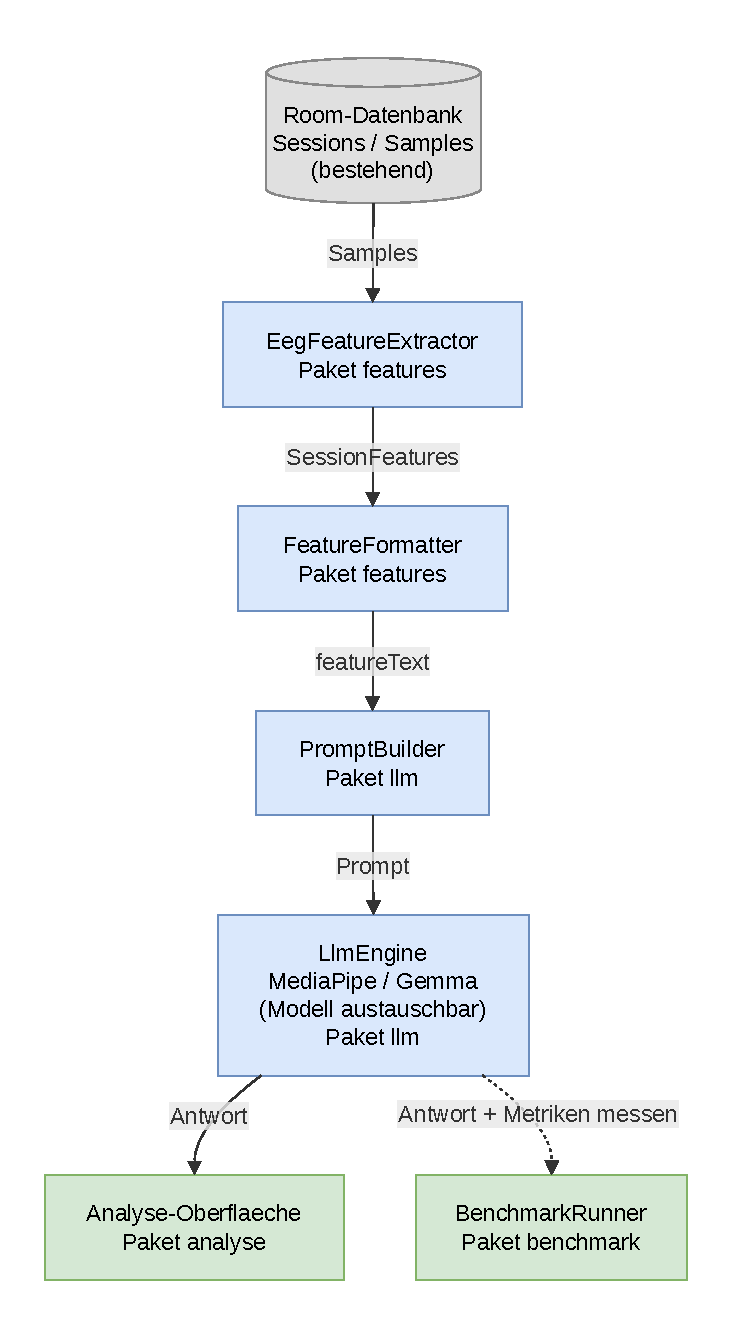
\includegraphics[width=0.6\textwidth]{Graphics/Projektarchitektur.drawio.pdf}
    \caption{Architektur und Datenfluss der Anwendung \autocite{drawio}}
    \label{fig:architektur}
\end{figure}

\begin{itemize}
\item \textbf{Datenbank:} Der Weg startet über die Datenbank, aus der die Samples abgerufen werden.
\item \textbf{EegFeatureExtractor:} Hier werden die Samples verarbeitet, indem Merkmale berechnet werden.
\item \textbf{FeatureFormatter:} Wandelt die Merkmale in ein für das Sprachmodell verständliches Format um.
\item \textbf{PromptBuilder:} Baut die Anweisung für den Prompt (je Szenario).
\item \textbf{LlmEngine:} Führt das Modell (Gemma via MediaPipe) aus und gibt die Antwort zurück.
\item \textbf{Analyse-Oberfläche:} Zeigt letztlich die Antwort an.
\item \textbf{Benchmark:} Misst die Verarbeitung (Laufzeit, Speicherverbrauch etc.).
\end{itemize}


\noindent Die Architektur ist in drei Kernbereiche unterteilt: zum einen das Paket \texttt{features}, das die Merkmalsextraktion übernimmt; zum anderen das Paket \texttt{llm}, das je nach Szenario den Aufbau des Prompts übernimmt und das Sprachmodell ausführt; und schließlich das Paket \texttt{analyse}, das die Benutzeroberfläche bereitstellt. Durch die Trennung dieser Pakete bleibt der Code übersichtlich, wartbar und erweiterbar.
\medskip

\noindent Ein zentrales Merkmal der Architektur ist die Kapselung des Sprachmodells in der Klasse \texttt{LlmEngine}. Die Klasse stellt eine einfache Schnittstelle bereit, die für das Laden, Anfragen und Freigeben verantwortlich ist. Dadurch wird die konkrete Modell- und Laufzeitumgebung vor dem Rest der Anwendung verborgen. Dies ermöglicht das Austauschen der Modelle, ohne dass die anderen Komponenten angepasst werden müssen.
In dieser Arbeit werden die Modelle Gemma 3 1B und Gemma 2 2B allein durch den Wechsel des Modellpfads auf dem mobilen Gerät geladen. Aus diesem Grund ließe sich an derselben Schnittstelle auch ein anderes Modell anbinden. Möglich wäre es auch, eine andere Laufzeitumgebung oder ein systemintegriertes Modell anzubinden. Diese Entkopplung ermöglicht es, die Anwendung flexibel und ohne großen Aufwand zu erweitern und zu warten.

\noindent Die in \autoref{fig:architektur} grün und blau markierten Komponenten stellen den eigenen Beitrag dar.

\section{Implementierung der Merkmalsextraktion}
\label{sec:impl-features}
Die Merkmalsextraktion ist im Paket \texttt{features} implementiert; zuständig dafür ist die Klasse \texttt{EegFeatureExtractor}. Sie durchläuft für jede Session eine feste Abfolge von Schritten: Als Erstes wird die Session aus der Datenbank geladen, daraufhin wird sie auf ihre Verwertbarkeit geprüft. Anschließend wird sie in gleich große Segmente aufgeteilt, bei denen dann jeweils die spektralen sowie statistischen Merkmale berechnet werden. Die Ergebnisse werden alle im Objekt \texttt{SessionFeatures} gesammelt und schließlich vom \texttt{FeatureFormatter} in einen lesbaren Text umgewandelt, den das Sprachmodell verarbeiten kann. Im Folgenden wird chronologisch auf die einzelnen Schritte genauer eingegangen.
\medskip

\noindent\textbf{Vorbereitung.} Sobald die Klasse erzeugt wird, werden vorab alle wiederverwendbaren Bestandteile angelegt (\autoref{lst:konstruktor}). Dazu gehört das Hann-Fenster, das für die Fourier-Transformation vorab berechnet wird, um bei jedem Fenster nicht erneut erzeugt zu werden. Außerdem wird das FFT-Objekt der Bibliothek JTransforms für die gewählte Fenstergröße instanziiert. Der Standardwert für die Fenstergröße beträgt 256, kann aber variabel angepasst werden. Aus ihr und der Anzahl der Segmente wird die Mindestlänge \texttt{minSamples} der Session berechnet.
\begin{lstlisting}[style=code, caption={Vorberechnung von Hann-Fenster und FFT-Objekt im Konstruktor}, label={lst:konstruktor}]
public EegFeatureExtractor(int windowSize) {
    this.windowSize = windowSize;
    this.hann       = hannWindow(windowSize);
    // Hann-Fenster vorberechnen
    this.fft        = new DoubleFFT_1D(windowSize);
    // FFT-Objekt aus JTransforms
    this.minSamples = windowSize * SEGMENT_COUNT;
}
\end{lstlisting}

\noindent\textbf{Validierung.} Die Methode \texttt{validate} prüft eine Session auf ihre Verwertbarkeit. Es gibt zwei Kriterien, die erfüllt sein müssen. Zum einen muss die Session mindestens so viele Samples enthalten, wie in \texttt{minSamples} berechnet wurde, ansonsten wird \texttt{TOO\_SHORT} zurückgegeben. Zum anderen muss der Anteil ungültiger Samples unter 50\,\% liegen. Ist dies nicht der Fall, wird \texttt{TOO\_MANY\_INVALID} zurückgegeben. Sind beide Kriterien erfüllt, wird die Analyse mit der Rückgabe von \texttt{OK} fortgesetzt, ansonsten wird dem Nutzer eine entsprechende Meldung angezeigt.
\begin{lstlisting}[style=code, caption={Vorabprüfung der Session}, label={lst:validate}]
public enum Check { OK, TOO_SHORT, TOO_MANY_INVALID; }

public Check validate(List<SampleEntity> samples) {
    if (samples == null || samples.size() < minSamples) {
        return Check.TOO_SHORT;
        // zu wenige Samples
    }
    int invalidCount = 0;
    for (SampleEntity sample : samples) {
        if (sample.valid == 0) invalidCount++;
    }
    if (invalidCount > MAX_INVALID_RATIO * samples.size()) {
        return Check.TOO_MANY_INVALID;
        // zu viele ungueltige Werte
    }
    return Check.OK;
}
\end{lstlisting}

\noindent\textbf{Segmentierung.} Die Methode \texttt{extract} stellt den Einstiegspunkt der Merkmalsextraktion dar. Dort wird die Session in \texttt{SEGMENT\_COUNT} gleich große Abschnitte (hier vier) zerlegt. Für jedes dieser Segmente werden separat die Merkmale (\autoref{lst:extract}) berechnet. Die Aufteilung in gleich große Stücke hilft dabei, den zeitlichen Verlauf innerhalb einer Session grob abzubilden, anstatt sie nur als ein einziges Mittel zu betrachten. Die einzelnen Segmente werden jeweils im \texttt{SessionFeatures}-Objekt abgelegt.
\begin{lstlisting}[style=code, caption={Zerlegung der Session in Segmente}, label={lst:extract}]
public SessionFeatures extract(List<SampleEntity> samples) {
    SessionFeatures features = new SessionFeatures();
    features.sessionId       = samples.get(0).sessionId;
    features.sampleCount     = samples.size();
    features.durationSeconds = samples.get(samples.size() - 1).sampleCounterSeconds;
    features.segments        = new ArrayList<>();

    int segLength = samples.size() / SEGMENT_COUNT;
    for (int i = 0; i < SEGMENT_COUNT; i++) {
        int start = i * segLength;
        int end   = (i == SEGMENT_COUNT - 1) ? samples.size() : start + segLength;
        List<SampleEntity> slice = samples.subList(start, end);
        features.segments.add(buildSegment(slice));
        // Merkmale pro Abschnitt berechnen
    }
    return features;
}
\end{lstlisting}

\noindent\textbf{Spektrale Merkmale (Welch-Methode).} Für jeden der acht EEG-Kanäle wird die Leistung in den Frequenzbändern Delta (\(\delta\)), Theta (\(\theta\)), Alpha (\(\alpha\)), Beta (\(\beta\)) und Gamma (\(\gamma\)) berechnet. Das geschieht nach dem Verfahren der Welch-Methode (\autoref{lst:bandpower}), bei der die Fourier-Transformation auf 50\,\% überlappende Segmente des Signals angewendet wird. Für jedes Fenster wird das Leistungsspektrum berechnet und in Bänder einsortiert, und über alle Fenster hinweg wird gemittelt. Durch die Mittelung wird ein stabileres Ergebnis geliefert, das weniger anfällig für zufällige Schwankungen ist.
\begin{lstlisting}[style=code, caption={Band-Power je Kanal nach dem Welch-Verfahren}, label={lst:bandpower}]
private double[][] computeBandPower(List<SampleEntity> slice) {
    double[][] result = new double[CHANNELS][NUM_BANDS];
    int hop = windowSize / 2;
    // 50% Ueberlappung

    for (int i = 0; i < CHANNELS; i++) {
        double[] signal = extractChannelSignal(slice, i);
        double[] bandAccum = new double[NUM_BANDS];
        int windowCount = 0;

        for (int start = 0; start + windowSize <= signal.length; start += hop) {
            double[] window = Arrays.copyOfRange(signal, start, start + windowSize);
            double[] power  = powerSpectrum(window);
            // Fenster -> Spektrum
            double[] bands  = sumBands(power);
            // Spektrum -> Baender
            for (int b = 0; b < NUM_BANDS; b++) bandAccum[b] += bands[b];
            windowCount++;
        }
        if (windowCount > 0) {
            for (int b = 0; b < NUM_BANDS; b++) {
                result[i][b] = bandAccum[b] / windowCount;
                // ueber alle Fenster mitteln (Welch)
            }
        }
    }
    return result;
}
\end{lstlisting}

\noindent Die Methode \texttt{powerSpectrum} berechnet das Leistungsspektrum eines Fensters (\autoref{lst:powerspectrum}). Zunächst wird der Mittelwert (Gleichanteil) abgezogen. Danach wird das Hann-Fenster angewendet, um anschließend die Fourier-Transformation durchzuführen. Schließlich wird die Leistung je Frequenz-Bin berechnet, indem die Real- und Imaginärteile quadriert und summiert werden.
\begin{lstlisting}[style=code, caption={Berechnung des Leistungsspektrums eines Fensters}, label={lst:powerspectrum}]
private double[] powerSpectrum(double[] window) {
    // 1. Mittelwert (Gleichanteil)
    double mean = 0;
    for (double v : window) mean += v;
    mean /= window.length;

    // 2. Mittelwert abziehen + Hann anwenden
    double[] data = new double[windowSize];
    for (int n = 0; n < windowSize; n++) {
        data[n] = (window[n] - mean) * hann[n];
    }

    // 3. FFT (in-place, JTransforms)
    fft.realForward(data);

    // 4. Leistung pro Frequenz-Bin
    double[] power = new double[windowSize / 2];
    power[0] = data[0] * data[0];
    // DC-Bin
    for (int k = 1; k < windowSize / 2; k++) {
        double re = data[2 * k], im = data[2 * k + 1];
        power[k] = re * re + im * im;
    }
    return power;
}
\end{lstlisting}

\noindent Die eigentliche Fourier-Transformation (\texttt{fft.realForward}) wird dabei durch die Bibliothek JTransforms bereitgestellt und nicht selbst implementiert \autocite{jtransforms}. Sie bietet eine Java-basierte Implementierung der Fourier-Transformation, die den Aufruf \texttt{realForward} für reelle Eingangssignale bereitstellt. Das Ergebnis wird dabei in dasselbe Array geschrieben, sodass die geraden Indizes die Real- und die ungeraden Indizes die Imaginärteile der Frequenz-Bins enthalten.
\medskip

\noindent\textbf{Zuordnung zu den Frequenzbändern.} Das Spektrum liefert die Leistung je Frequenz-Bin. Diese müssen noch den Frequenzbändern zugeordnet werden (\autoref{lst:sumbands}). Dazu wird jeder Bin-Index über die Beziehung \(\text{freq} = i \cdot f_s / N\) in eine Frequenz umgerechnet. Der Faktor \(f_s / N\) entspricht dabei der Frequenzauflösung \(\Delta f\) (\autoref{eq:freqaufloesung}), also dem Frequenzabstand zwischen zwei benachbarten Bins. Dadurch können für jedes Frequenzband die entsprechenden Bins summiert werden.
\begin{lstlisting}[style=code, caption={Zuordnung der Frequenz-Bins zu den Bändern}, label={lst:sumbands}]
private double[] sumBands(double[] power) {
    double[] bandSum = new double[NUM_BANDS];
    for (int i = 1; i < power.length; i++) {
        double freq = (double) (i * SAMPLE_RATE) / windowSize;
        // Bin-Index -> Frequenz
        for (FrequencyBand band : FrequencyBand.values()) {
            if (freq >= band.lowHz && freq < band.highHz) {
                bandSum[band.ordinal()] += power[i];
            }
        }
    }
    return bandSum;
}
\end{lstlisting}

\noindent Die Einteilung in die jeweiligen Frequenzbänder wird durch den Aufzählungstyp (\texttt{enum}) \texttt{FrequencyBand} realisiert, der als zentrale Definitionsstelle der Bänder dient (\autoref{lst:frequencyband}). Jedes Band ist dort mit seiner unteren und oberen Grenzfrequenz hinterlegt.
\begin{lstlisting}[style=code, caption={Zentrale Definition der Frequenzbänder mit ihren Grenzen}, label={lst:frequencyband}]
public enum FrequencyBand {
    DELTA(0.5f, 4f),
    THETA(4f,   8f),
    ALPHA(8f,   13f),
    BETA(13f,   30f),
    GAMMA(30f,  45f);

    public final float lowHz;
    public final float highHz;

    FrequencyBand(float lowHz, float highHz) {
        this.lowHz  = lowHz;
        this.highHz = highHz;
    }
}
\end{lstlisting}

\noindent\textbf{Statistische Merkmale.} Als erstes der zwei statistischen Merkmale wird der Peak-to-Peak-Wert berechnet. Dieser stellt die Spannweite je Kanal dar. Er beschreibt die Differenz zwischen dem höchsten und dem niedrigsten Messwert. Dadurch sind starke Ausschläge oder Drift sichtbar. Der zweite statistische Wert ist der Anteil der ungültigen Samples (\texttt{valid == 0}) an der Gesamtzahl im Segment. Er dient als Maß für die Signalqualität.
\medskip

\noindent\textbf{Ergebnis.} Abschließend werden die berechneten Merkmale in einem Objekt \texttt{SessionFeatures} gesammelt. Dieses dient als Datencontainer, der alle Daten der Session sowie die Liste der Segmente mit ihren Merkmalen enthält. Das Ergebnis dieser Schritte ist die Grundlage für die anschließende Aufbereitung durch den \texttt{FeatureFormatter}.


\section{Integration des Sprachmodells}
\label{sec:impl-llm}
% TODO: MediaPipe, Modell-Handling, LlmEngine

\section{Prompt-Design und iterative Optimierung}
\label{sec:impl-prompt}
Wie schon in \autoref{sec:szenarien} erwähnt, besteht der Prompt aus den aufbereiteten Merkmalen mit einer szenariospezifischen Anweisung. Dieser ist für alle Modelle identisch.
Der Prompt wurde in der Klasse \texttt{PromptBuilder} realisiert. Der Weg bis zum finalen Prompt war iterativ: Er wurde anhand der Modellausgaben verfeinert und anschließend für die Evaluation final festgehalten.
\medskip

\noindent Bei der Optimierung des Prompts ergaben sich folgende Design-Vorgaben, die jeweils auf ein beobachtetes Problem der frühen Ausgaben zurückgehen:
\begin{itemize}
\item \textbf{Datentreue:} Es wird darauf hingewiesen, nur die Werte zu verwenden, die genannt werden. Dies soll verhindern, dass das Modell eigene Annahmen trifft. Dieses Problem trat in früheren Ausgaben auf, so wurden Begriffe wie \enquote{Dominanzindex} genannt.
\item \textbf{Reines Textformat:} Es wird sichergestellt, dass die Ausgaben des Modells nur textuelle Informationen enthalten. Es werden Sonderzeichen (Markdown) verboten, da sonst Formatierungszeichen (z.,B. \texttt{**}) auftraten.
\item \textbf{Eindeutige Merkmalsbenennung:} Im \texttt{FeatureFormatter} wird der Anteil ungültiger Werte als \enquote{Ungültige Messwerte: X\,\%} statt als \enquote{Qualität: X\,\%} ausgegeben. Zuvor interpretierte das Modell \enquote{Qualität: X\,\%} fälschlich als schlechte Qualität.
\item \textbf{Begrenzung der Interpretation:} Ausgaben mit falscher Interpretation, etwa durch die Einbeziehung medizinischer Diagnosen, werden verhindert, da sie zuvor ein Problem darstellten.
\item \textbf{Kompaktheit:} Wenige Sätze, keine Begrüßung oder Rückfragen.
\end{itemize}

\noindent Nach der Optimierung wurde der finale Prompt eingefroren und für alle Messungen verwendet. Er stellt auch die Grundlage für den Benchmark dar. In \autoref{lst:prompts} sind die finalen Prompts je Szenario dargestellt.
\begin{lstlisting}[language=Java, framextopmargin=5pt, framexbottommargin=5pt, xleftmargin=5pt, xrightmargin=5pt, basicstyle=\footnotesize\ttfamily, breaklines=true, caption={Aufbau der Prompts je Szenario (finale, eingefrorene Fassung)}, label={lst:prompts}]
    // Szenario 1: Session-Report
public String buildReport(String featureText) {
    
    return "Fasse die folgenden EEG-Messwerte in 3 bis 4 Saetzen sachlich zusammen. "
         + "Schreibe nur den Bericht: keine Begruessung, keine Rueckfragen, kein Schlusssatz. "
         + "Schreibe reinen Fliesstext ohne Sonderzeichen (kein Markdown). "
         + "Nenne das dominante Frequenzband, die Signalqualitaet und auffaellige Ausschlaege. "
         + "Erfinde nichts und nutze nur die folgenden Werte:\n\n"
         + featureText;
}

// Szenario 2: Artefakt-Erklaerung
public String buildArtefaktErklaerung(String featureText) {
    
    return "Analysiere die folgenden EEG-Messwerte und beziehe dich konkret auf die genannten Werte. "
         + "Benenne die auffaelligsten Punkte dieser Session (z. B. sehr hohe Ausschlaege, "
         + "ungueltige Daten oder ein stark dominantes Band) und erklaere kurz ihre moegliche "
         + "technische Ursache (z. B. Bewegung, Elektroden, Verbindung). Stelle keine "
         + "medizinischen Diagnosen. Schreibe wenige Saetze als sachlichen Fliesstext, ohne "
         + "Begruessung und ohne Sonderzeichen (kein Markdown). Erfinde nichts und nutze nur "
         + "die folgenden Werte:\n\n"
         + featureText;
}

// Szenario 3: Session-Vergleich
public String buildVergleich(String featureTextA, String featureTextB) {
    
    return "Vergleiche die folgenden zwei EEG-Sessions und beschreibe die wichtigsten "
         + "Unterschiede in einfachen Worten (z. B. Banddominanz, Signalqualitaet, Ausschlaege). "
         + "Schreibe sachlichen Fliesstext ohne Sonderzeichen (kein Markdown). Erfinde keine "
         + "Kennzahlen oder Begriffe. Schreibe nur den Vergleich, keine Begruessung. "
         + "Nutze nur die folgenden Werte.\n\n"
         + "Session A:\n" + featureTextA
         + "\n\nSession B:\n" + featureTextB;
}
\end{lstlisting}


\section{Benutzeroberfläche}
\label{sec:impl-ui}
% TODO: KI-Analyse-Screen (kurz)
\cleardoublepage\chapter{Evaluation}
\label{ch:evaluation}
Dieses Kapitel präsentiert die Durchführung (\autoref{subsec:messbedingungen}) sowie die Ergebnisse der Metriken (\autoref{subsec:metriken}), um zu beurteilen, inwiefern sich die lokalen Modelle für die Verarbeitung von EEG-Daten eignen.

\section{Durchführung der Messungen}
\label{sec:eval-durchfuehrung}
Wie schon in \autoref{sec:messprotokoll} beschrieben, wird die Eingabe für alle Modelle identisch gehalten. Insgesamt werden so alle neun Kombinationen aus drei Modellen und drei Szenarien auf dem Samsung Galaxy S23 vermessen und anschließend in einer neu erstellten CSV-Datei protokolliert. Dies geschieht je fünfmal, wobei die erste Messung jeder Kombination verworfen wird.
Vor der ersten Messung wird ein Aufwärmlauf durchgeführt.
\medskip

\noindent Als Eingabe für das Modell werden zwei bestimmte Sessions verwendet. Beide sind beim Tragen des Unicorn-Hybrid-Headsets entstanden und haben eine Laufzeit von knapp über 120 Sekunden.
% Kurzer Recap (kein Wiederholen der ganzen Methodik):
% - 3 Modelle x 3 Szenarien, N=5, erste Messung verworfen
% - Bedingungen -> \autoref{subsec:messbedingungen}
% - Testgerat S23
% 3-4 Satze reichen.

\section{Latenz}
\label{sec:eval-latenz}
Im folgenden werden die Ergebnisse der Latenzmessungen vorgestellt.
% Deutung: welches Modell schneller? TTFT vs Gesamtdauer? Tokens/s als fairer Vergleich.
\setlength{\tabcolsep}{4pt}
\begin{table}[H]
    \centering
    \caption{Latenzmetriken je Modell und Szenario (Mittel aus vier Wiederholungen $\pm$ Standardabweichung).}
    \label{tab:eval-latenz}
    \begin{tabular}{llrrrr}
        \toprule
        \textbf{Modell} & \textbf{Szenario} & \textbf{Ladezeit (s)} & \textbf{TTFT (s)} & \textbf{Gesamtdauer (s)} & \textbf{Tok/s} \\
        \midrule
        \multirow{3}{*}{Gemma 3 1B}
            & Report    & 0,45 & 1,94 $\pm$ 0,07 & 6,70 $\pm$ 0,14  & 21,65 $\pm$ 0,44 \\
            & Artefakt  & 0,34 & 1,95 $\pm$ 0,04 & 11,44 $\pm$ 0,04 & 25,34 $\pm$ 0,09 \\
            & Vergleich & 0,29 & 5,86 $\pm$ 0,49 & 9,89 $\pm$ 0,46  & 11,85 $\pm$ 0,54 \\
        \midrule
        \multirow{3}{*}{Qwen 2.5 1.5B}
            & Report    & 0,73 & 5,36 $\pm$ 0,10 & 34,43 $\pm$ 0,24 & 14,06 $\pm$ 0,10 \\
            & Artefakt  & 0,27 & 5,31 $\pm$ 0,13 & 26,70 $\pm$ 0,12 & 13,37 $\pm$ 0,06 \\
            & Vergleich & 0,27 & 13,99 $\pm$ 0,55 & 42,00 $\pm$ 1,94 & 11,31 $\pm$ 0,53 \\
        \midrule
        \multirow{3}{*}{Gemma 2 2B}
            & Report    & 0,87 & 6,09 $\pm$ 0,49 & 14,25 $\pm$ 0,49 & 5,06 $\pm$ 0,17 \\
            & Artefakt  & 0,47 & 6,75 $\pm$ 0,38 & 18,57 $\pm$ 0,58 & 4,74 $\pm$ 0,15 \\
            & Vergleich & 0,52 & 16,60 $\pm$ 0,23 & 27,19 $\pm$ 0,13 & 2,87 $\pm$ 0,01 \\
        \bottomrule
    \end{tabular}
\end{table}

\noindent \autoref{tab:eval-latenz} zeigt, dass der \textbf{Durchsatz (Tok/s)} bei dem Modell Gemma 3 1B am höchsten ist (bis zu 25,34 Tok/s), während das Modell Gemma 2 2B den geringsten Durchsatz aufweist (minimal 2,87 Tok/s).
Die \textbf{Ladezeit} ist bei Gemma 2 2B am höchsten; die beiden kleineren Modelle Gemma 3 1B und Qwen 2.5 1.5B laden schneller. Sie liegt durchweg unter einer Sekunde (zwischen 0,27 und 0,87,s).
Die \textbf{Zeit bis zum ersten Token (TTFT)} ist bei Gemma 3 1B am geringsten, während sie bei Gemma 2 2B am höchsten ist. Mit Ausnahme von Qwen 2.5 1.5B/Artefakt steigt die TTFT mit dem Szenarioniveau an und erreicht ihren Höchstwert bei Gemma 2 2B mit 16,60,s.
Die \textbf{Gesamtdauer} reicht von etwa 6,70 bis 42,00,s und variiert stark zwischen den Modellen und Szenarien.
\medskip

\noindent Da die \textbf{Standardabweichungen} überwiegend gering ausfallen, weisen sie auf stabile Messungen hin. Lediglich bei Qwen 2.5 1.5B/Vergleich ist die Standardabweichung mit 1,94,s (Gesamtdauer) deutlich höher als bei allen anderen Messungen.
\section{Ressourcenverbrauch}
\label{sec:eval-ressourcen}
Daraufolgend werden die Ergebnisse der Messungen zum Ressourcenverbrauch vorgestellt.
% Deutung: RAM waechst mit Modellgroesse? Akku-Tradeoff (2B ~1,5x 1B, aus deinem 1. Lauf).

\begin{table}[H]
    \centering
    \caption{Ressourcenverbrauch je Modell (RAM als Mittel $\pm$ Standardabweichung).}
    \label{tab:eval-ressourcen}
    \begin{tabular}{llrr}
        \toprule
        \textbf{Modell} & \textbf{Szenario} & \textbf{RAM / PSS (MB)} & \textbf{Akku (mAh)\textsuperscript{*}} \\
        \midrule
        \multirow{3}{*}{Gemma 3 1B}
            & Report    & 1482 $\pm$ 43 & \multirow{3}{*}{\textasciitilde70} \\
            & Artefakt  & 1508 $\pm$ 10 & \\
            & Vergleich & 1615 $\pm$ 35 & \\
        \midrule
        \multirow{3}{*}{Qwen 2.5 1.5B}
            & Report    & 1994 $\pm$ 2  & \multirow{3}{*}{\textasciitilde200} \\
            & Artefakt  & 1994 $\pm$ 1  & \\
            & Vergleich & 2114 $\pm$ 34 & \\
        \midrule
        \multirow{3}{*}{Gemma 2 2B}
            & Report    & 3691 $\pm$ 129 & \multirow{3}{*}{\textasciitilde100} \\
            & Artefakt  & 3638 $\pm$ 168 & \\
            & Vergleich & 3798 $\pm$ 128 & \\
        \bottomrule
    \end{tabular}
    \\[4pt]
    \footnotesize\textsuperscript{*}Verbrauch über den gesamten Messblock (15 Läufe) des jeweiligen Modells.
\end{table}

\noindent \autoref{tab:eval-ressourcen} zeigt, dass der \textbf{RAM (PSS)} eine klare Rangfolge zwischen den Modellen besitzt. Während Gemma 3 1B mit (1482 MB) den geringsten Wert aufweist, liegt Qwen in der Mitte (ca.\ 2000 MB) und Gemma 2 2B am höchsten (3798 MB).
Während das 1B-Modell von Gemma mit (ca.\ 70 mAh) den geringsten \textbf{Akkuverbrauch} aufweist, liegt der Verbrauch von Qwen 2.5 1.5B (ca.\ 200 mAh) und Gemma 2 2B (ca.\ 100 mAh) deutlich höher.
Auffällig ist, dass das Modell Qwen am meisten Akku verbraucht.
\section{Stabilität}
\label{sec:eval-stabilitaet}
Alle 45 Messungen wurden mit dem Status \enquote{ok} protokolliert. Das bedeutet, dass alle Läufe erfolgreich liefen. Es gab keine Abstürze, keine Fehler und keinen Speicherüberlauf ().
Das größere Modell Gemma 2 2B lief ebenso stabil, obwohl es mit ca.\ 3742,MB den meisten RAM verbrauchte.
Auffällig war lediglich eine leichte Schwankung, die bei Gemma 2 2B/Artefakt auftrat. Dort fiel eine größere Streuung auf (± 2,24,s), die vermutlich unter Dauerlast entstand.
% Status-Verteilung (erfolgreich/Fehler/OOM), Throttling-Beobachtungen,
% ob ein Modell an die RAM-Grenze des S23 kam. Meist Fliesstext + evtl. kleine Tabelle.

\section{Ausgabequalität}
\label{sec:eval-qualitaet}
% Qualitative Bewertung. Erst Kriterien definieren, dann Beispielausgaben einordnen.

\subsection{Bewertungskriterien}
\label{subsec:eval-kriterien}
\begin{itemize}
    \item \textbf{Korrektheit:} Stimmt die Aussage mit den Merkmalen überein?
    \item \textbf{Verständlichkeit:} Ist die Ausgabe für Laien lesbar?
    \item \textbf{Relevanz:} Geht sie auf das Wesentliche ein?
    \item \textbf{Halluzination:} Werden Dinge erfunden, die nicht in den Daten stehen?
\end{itemize}

\subsection{Beispielausgaben je Szenario}
\label{subsec:eval-beispiele}
% Pro Szenario 1-2 Beispielausgaben (z.B. als \begin{quote} oder lstlisting)
% + kurze Einordnung anhand der Kriterien oben.
% Szenario 1: Session-Report
% Szenario 2: Artefakt-Erklarung
% Szenario 3: Session-Vergleich

\section{Zusammenfassende Gegenüberstellung}
\label{sec:eval-vergleich}
% Ein Gesamtbild: welches Modell fuer welchen Zweck? Tabelle oder Ampel-Uebersicht.
% Ueberleitung zur Diskussion (\autoref{ch:diskussion}).
\cleardoublepage\chapter{Diskussion}
\label{ch:diskussion}
Nun werden die Ergebnisse der Evaluation eingeordnet. Danach folgen die Einschränkungen der Arbeit und Handlungsempfehlungen für den praktischen Einsatz lokaler Sprachmodelle in mobilen BCI-Anwendungen.

\section{Einordnung der Ergebnisse}
\label{sec:einordnung}
Die verwendeten Gemma-Modelle unterscheiden sich in ihren Stärken. Gemma 3 1B ist aufgrund seiner geringen Größe am effizientesten und hat den geringsten Speicher- und Akkubedarf sowie die höchste Geschwindigkeit. Das liegt daran, dass die Modellgröße einen Einfluss auf den Speicher- und Rechenaufwand hat (\autoref{subsec:ondevice}). Gemma 2 2B liegt innerhalb der beiden Gemma-Modelle an erster Stelle, wenn man allein die Ausgabequalität betrachtet.
\vspace{\baselineskip}

\noindent Qwen 2.5 1.5B zeigt, dass die Größe allein die Qualität nicht bestimmt. Obwohl es sich von der Parameterzahl her in der Mitte der drei Modelle einordnet, liefert es die schlechtesten Ausgaben. Die technischen Bedingungen waren für alle Modelle gleich (\autoref{ch:methodik}).
Qwen 2.5 1.5B hat die höchste Inferenzdauer und verbraucht am meisten Akku, obwohl es kleiner als Gemma 2 2B ist. Das Modell pendelt sich aber bei dem Rest, bis auf die Ladezeit im Artefakt- und Vergleichsszenario, bei der es mit 0,27\,s am schnellsten ist, in der Mitte ein. Der Grund für die lange Inferenzdauer liegt in der Länge der Antworten. Je mehr Text ein Modell erzeugt, desto länger dauert die Berechnung und desto mehr Energie verbraucht sie. Qwen 2.5 1.5B erzeugt in den Messungen deutlich mehr Tokens (vgl.\ \autoref{tab:app-rohdaten}). Wenn man den Durchsatz von Qwen 2.5 1.5B betrachtet, liegt er mit 11,31 bis 14,06 Tokens pro Sekunde in einem deutlich schnelleren Bereich als Gemma 2 2B mit 2,87 bis 5,06 (\autoref{tab:eval-latenz}). Qwen 2.5 1.5B erzeugt seine Tokens also nicht langsamer, sondern nur mehr davon. Die Ausführlichkeit ist gleichzeitig ein Qualitätsproblem, weil es sich schlecht an die Vorgaben hält. Trotz der klaren Formatvorgaben im Prompt fällt die Antwort zu lang aus. Die Ausgabe ist so nicht nur inhaltlich am schwächsten, sondern kostet auch am meisten Zeit und Energie. Beides tritt bei Qwen gemeinsam auf, möglicherweise durch das Nichteinhalten der Längenvorgaben oder eine ungeeignete Promptwahl. Ein fester Zusammenhang lässt sich jedoch aus den Messungen nicht ableiten.
\vspace{\baselineskip}

\noindent Die \ac{TTFT} ist im Vergleichsszenario bei allen drei Modellen deutlich länger als bei Report und Artefakt-Erklärung. Das liegt an der längeren Prompteingabe, bei der gleich zwei Merkmalstexte (einer je Session) verarbeitet werden. Je mehr Text ein Modell liest, desto länger dauert es bei diesem Modell in der Regel, bis die Antwort generiert wird. Dies bestätigt sich in den Eingabe-Tokenzahlen (\autoref{tab:eval-eingabetokens}), die im Vergleichsszenario am größten ausfallen. Wichtig zu erwähnen ist, dass Qwen 2.5 1.5B den Prompt in allen Szenarien in die meisten Tokens zerlegt. Der Zerlegungsunterschied zwischen den Modellen kann durch das kleinere Vokabular von Qwen 2.5 1.5B (\autoref{subsec:messbedingungen}) entstehen, ebenso können die abweichenden Zerlegungsverfahren oder die Struktur des Prompts die Ursache sein. Welcher dieser Einflüsse überwiegt, bleibt offen, da es aus den Daten nicht sicher abgeleitet werden kann. Da die Tokenanzahl der Eingabe gegenüber Gemma 3 1B nur wenige Prozent (4 bis 8) höher ist, lässt sich die im Verhältnis klar erhöhte \ac{TTFT} von Qwen 2.5 1.5B nicht mit der Länge der Eingabe erklären. Gemma 2 2B erreicht mit nahezu gleich vielen Eingabe-Tokens wie Gemma 3 1B sogar die höchste \ac{TTFT}. Damit begründet sich der Unterschied zwischen den Modellen wahrscheinlich durch den erhöhten Rechenaufwand (\autoref{subsec:ondevice}). Innerhalb eines Modells können die Eingabe-Tokens einen Einfluss auf die \ac{TTFT} haben, zwischen den Modellen erklären sie die Unterschiede jedoch nicht. Eine Ausnahme zeigt sich bei Qwen 2.5 1.5B im Artefakt-Szenario, wo die \ac{TTFT} trotz mehr Eingabe-Tokens leicht unter dem Report-Szenario liegt. Der Unterschied ist mit 0,05\,s aber sehr gering und liegt innerhalb der Standardabweichung (\autoref{tab:eval-latenz}).
\vspace{\baselineskip}

\noindent Die Tokens pro Sekunde werden direkt von der längeren Vorlaufzeit beeinflusst. Die Metrik ergibt sich aus den erzeugten Tokens geteilt durch die gesamte Inferenzdauer (\autoref{subsec:metriken}), bei der die \ac{TTFT} einen großen Anteil ausmachen kann. So entfallen im Vergleichsszenario bei Gemma 3 1B rund 59 Prozent und bei Gemma 2 2B rund 61 Prozent der Inferenzdauer auf die Phase vor dem ersten Token, im Report-Szenario sind es 29 beziehungsweise 43 Prozent. Da bei Qwen 2.5 1.5B der Anteil aufgrund der längeren Ausgaben im Report- und Vergleichsszenario bei nur 16 beziehungsweise 33 Prozent liegt, fällt dort auch der Durchsatz am wenigsten ab. \autoref{tab:eval-latenz} zeigt, dass sich der Durchsatz vom Report- zum Vergleichsszenario bei dem Modell Gemma 3 1B von 21,65 auf 11,85 Tokens pro Sekunde fast halbiert. So auch bei Gemma 2 2B, bei dem der Durchsatz von 5,06 auf 2,87 sinkt. Bei Qwen 2.5 1.5B sinkt er nur von 14,06 auf 11,31 Tokens pro Sekunde. Dass der Rückgang an der Vorlaufzeit liegt, zeigt sich, wenn man sie herausrechnet. Dann bleibt die reine Erzeugungsrate weitgehend gleich, bei Gemma 3 1B 30,5 gegenüber 29,0 und bei Qwen 2.5 1.5B 16,7 gegenüber 16,9 Tokens pro Sekunde. Spürbar sinkt sie nur bei Gemma 2 2B, von 8,8 auf 7,4, da sich die Werte relativ zueinander um rund 16 Prozent unterscheiden. Der Einbruch geht damit vor allem auf die längere Verarbeitung der Eingabe zurück. Die Ladezeit liegt im Bereich von 0,27 bis 0,87\,s bei allen Modell-Szenario-Kombinationen und fällt daher gegenüber der bis zu 42\,s langen Inferenzdauer kaum ins Gewicht (\autoref{tab:eval-latenz}).
\vspace{\baselineskip}

\noindent Durch den Verbrauch in \ac{PSS} kann man den von der Anwendung benutzten \ac{RAM} ins Verhältnis zum gesamten \ac{RAM} von 8 GB setzen. Gemma 2 2B belegt mit ca.\ 3,7 GB rund 45 Prozent der verfügbaren 8 GB, Gemma 3 1B mit ca.\ 1,5 GB rund 18 Prozent und Qwen 2.5 1.5B mit ca.\ 2,0 GB rund 24 Prozent. Bei dem 2B-Modell wären es auf einem Gerät mit 4 GB Arbeitsspeicher ca.\ 90 Prozent und damit an der Grenze. Da der \ac{PSS}-Wert eine obere Schranke darstellt (\autoref{subsec:metriken}), sind dies Höchstwerte. Zu beachten ist, dass einer Anwendung nie der gesamte Arbeitsspeicher netto zur Verfügung steht, da das System den Speicher unter Systemprozessen und Anwendungen aufteilt und bei Knappheit Prozesse beendet \autocite{android_memory}. Daraus lässt sich ableiten, dass 4 GB für das 2B-Modell sehr wahrscheinlich zu klein wären. Wahrscheinlich sind 6 GB oder 8 GB das Mindestmaß, das für das 2B-Modell benötigt wird. Geräte mit mehr \ac{RAM} können je nach Kompatibilität, Hardware und Android-Version größere Modelle verwenden.
\vspace{\baselineskip}

\noindent Mögliche Gründe für das schlechte Einhalten der Vorgaben bei Qwen lassen sich aus den Messungen allein nicht klären. Das Kontextfenster ist ausgeschlossen, da selbst im Vergleichsszenario mit 770 Eingabe- und 474 Ausgabe-Tokens die Grenze von 1280 Tokens nicht erreicht wird (\autoref{tab:app-rohdaten}). Wahrscheinlich liegt es an der Feinjustierung des Prompts, die speziell an das Modell Gemma 2 2B angepasst wurde (\autoref{sec:einschraenkungen}). Denkbar ist zudem, dass sich die Modelle darin unterscheiden, wie strikt sie Längen- und Formatvorgaben umsetzen.
\vspace{\baselineskip}

\noindent Hinzu kommt, dass Qwen 2.5 1.5B einen größeren Nachteil hat als die Gemma-Modelle. Gemma 3 1B kommt aus derselben Modellfamilie wie der Vorgänger und hat dadurch wahrscheinlich einen größeren Mehrwert durch die Prompt-Feinjustierung des Vorgängers. Qwen kommt von einem anderen Hersteller mit einem eigenen Tokenizer (\autoref{sec:qwen}), wodurch eine negative Beeinflussung nicht ausgeschlossen ist. Es kann auch sein, dass Qwen gegenüber den verwendeten Gemma-Modellen eine 8-Bit-Quantisierung und den Standardwert der Temperatur anders verarbeitet (\autoref{subsec:ondevice}, \autoref{sec:modellauswahl}). Die schwächeren Ergebnisse von Qwen sind daher nicht allein als geringere Fähigkeit zu lesen, sondern zum Teil als Folge eines Prompts, der nicht auf dieses Modell abgestimmt ist, und möglicherweise der Quantisierung oder der Temperatur.
\vspace{\baselineskip}

\noindent Die Ergebnisse zeigen somit, dass sich von der Modellgröße nicht unmittelbar auf die Ausgabequalität schließen lässt. Verschiedene Hersteller unterscheiden sich in Aufbau und Training der Modelle \autocite{gemma2_2024, qwen2025}, sodass die Größe als Anhaltspunkt nicht verlässlich genug ist. Bei der Stabilität unterscheiden sich die Modelle hingegen nicht. Alle Kombinationen laufen fehlerfrei durch. Die Feststellung in \autoref{sec:eval-latenz}, dass die Ausgabe immer identisch ist, liegt am Zufallsstartwert der Schnittstelle (\autoref{sec:modellauswahl}). Nur Qwen 2.5 1.5B weist einen erhöhten Streuungswert im Vergleichsszenario auf, was mit seiner langen Laufzeit unter Dauerlast zusammenhängen kann. Für die Forschungsfrage ist das Wichtigste, dass die Modelle einwandfrei und stabil ihre Aufgaben erfüllen und einen Mehrwert bieten. Solange die Latenz in einem vertretbaren Rahmen liegt, ist die Ausgabequalität das wichtigste Kriterium. Ob das hier bei den genutzten Modellen zutrifft, lässt sich nur vermuten.

\section{Einschränkungen}
\label{sec:einschraenkungen}
Während der gesamten Arbeit gibt es Einschränkungen, die die Ergebnisse beeinflussen können. Dazu gehören unter anderem Limitierungen durch Hardware, Designentscheidungen oder Entscheidungen bezogen auf die Messungen.
Die Arbeit basiert auf nur einem Testgerät, dem Samsung Galaxy S23. Es ist nicht sicher, wie die Evaluation auf anderen Hardwarekonfigurationen ausfallen würde. Das Testgerät schränkt zudem die Auswahl der Modelle ein. Aufgrund seiner begrenzten Unterstützung ist es nicht möglich, systemintegrierte Modelle wie Gemini Nano einzubeziehen \autocite{mlkit_genai_devices}. Zwar unterstützt das Testgerät Galaxy AI, dabei handelt es sich jedoch um vordefinierte Endnutzerfunktionen \autocite{samsung_galaxyai} und nicht um eine Schnittstelle, über die eigene Prompts an ein Sprachmodell übergeben werden könnten. Für den hier untersuchten Anwendungsfall ist es deshalb nicht einsetzbar. Auch bei den frei deploybaren Modellen ist die Auswahl begrenzt. Durch die selbst getroffene Wahl von MediaPipe als Laufzeitumgebung entfallen viele neuere Modelle, da die Schnittstelle nur eine begrenzte Auswahl unterstützt \autocite{mediapipe_llm} oder die Modelle für mobile Geräte gar nicht optimiert sind \autocite{edgellm_review}. Zudem wird für einen technisch einheitlichen Vergleich darauf geachtet, dass alle mit einer Kontextgröße von 1280, einer 8-Bit-Quantisierung und dem .task-Format laufen, was zur Folge hat, dass noch mehr Modelle ausgeschlossen werden.
\vspace{\baselineskip}

\noindent Die gesamte Promptfeinjustierung basiert auf dem Modell Gemma 2 2B, wodurch das Setup auf dieses Modell zugeschnitten ist. Davon betroffen ist sehr wahrscheinlich die Ausgabequalität sowie aufgrund der Länge der Ausgabe die Inferenzdauer, der Durchsatz und der Akkuverbrauch. Da die betroffenen Werte als Ergebnis unter günstigen Bedingungen entstanden sind, stellt sich die Frage, ob Gemma 2 2B in den Vergleich gezogen werden soll. Da Ladezeit, \ac{TTFT} und Speicherbedarf davon unberührt bleiben, wird das Modell im Vergleich belassen. Die betroffenen Werte sind jedoch entsprechend einzuordnen. Der Zuschnitt wirkt zudem nicht nur auf Gemma 2 2B. Da Gemma 3 1B derselben Modellfamilie angehört, dürfte es von der Feinjustierung teilweise mitprofitieren, während Qwen 2.5 1.5B als Modell eines anderen Herstellers keinen solchen Vorteil hat.\vspace{\baselineskip}

\noindent Beim Messaufbau ist die Reihenfolge der Messungen bewusst festgelegt (\autoref{sec:messprotokoll}). Trotz einer Abkühlphase lässt sich nicht ausschließen, dass die zuletzt gemessenen Modelle durch das wärmere Gerät leicht benachteiligt werden (\autoref{subsec:ondevice}). Dasselbe gilt für den Ladezustand, der über die Messreihe hinweg sinkt. Die Streuung der Zeiten geht deshalb auf die Messumgebung zurück. Der verbleibende Einfluss bleibt offen. Alle Messungen erfolgen zudem in deutscher Sprache, daher bleibt es offen, wie sich die Ausgabequalität und Tokenanzahl in englischer Sprache verhalten. Schließlich sind die drei Szenarien in ihrer Aufgabenart identisch, nämlich in der textuellen Beschreibung von \ac{EEG}-Sessions (\autoref{sec:szenarien}). Der Unterschied liegt im Anspruch und nicht in der Art der Aufgabe. Daher bleibt es offen, wie die Modelle bei anderen Aufgaben wie der Klassifikation abschneiden würden.
\vspace{\baselineskip}

\noindent Wie in \autoref{subsec:aufbereitung} beschrieben, wächst der Aufwand der Merkmalsextraktion linear mit der Länge der Session. Die Inferenzdauer ist davon nicht beeinflusst, da unabhängig von der Länge immer vier Segmente entstehen. Bei längeren Sessions von vielen Minuten könnte sich ihr Einfluss deutlich erhöhen und die Extraktion stärker ins Gewicht fallen.

\section{Handlungsempfehlungen}
\label{sec:empfehlungen}
In diesem Abschnitt werden Handlungen auf Basis der Erkenntnisse dieser Arbeit empfohlen. Diese leiten sich aus den Ergebnissen der Evaluation und aus der Umsetzung ab. Die folgenden Empfehlungen gelten für den in dieser Arbeit untersuchten Rahmen, also für die beschriebene Implementierung mit der in \autoref{sec:impl-prompt} festgelegten Prompt-Struktur und der gewählten Konfiguration, für die drei Anwendungsszenarien aus \autoref{sec:szenarien} und für das Testgerät aus \autoref{subsec:messbedingungen}. Auf andere Geräte, Prompts oder Aufgaben lassen sie sich nicht ohne Weiteres übertragen.

\subsection{Allgemeine Empfehlungen}
Die Prompts sollten im besten Fall kurz und klar gehalten werden, damit sie in den Kontext passen. Die Länge beeinflusst ebenso die Zeit bis zum ersten Token (\autoref{sec:einordnung}).
Das Modell sollte die Merkmale in einer klar verständlichen Form erhalten, ohne selbst überfordert zu sein, also keine Rohdaten, sondern aggregierte Merkmale.
Darüber hinaus sollte man je nach Szenario das passende Modell auswählen, da die Ausgabequalität je nach Komplexität der Aufgabe variiert.
Da die Modelle jeweils 1,5\,GB, 2,0\,GB und 3,7\,GB im Arbeitsspeicher belegen (\autoref{tab:eval-ressourcen}), sollten sie erst nach der Prüfung der Eingabe geladen werden. Nach der Ausgabe können sie schließlich wieder freigegeben werden.
Die Inferenz der Modelle sollte auf einen Hintergrund-Thread verlagert werden, da eine Anfrage bis zu 42\,s dauern kann und die Oberfläche einfrieren würde (\autoref{tab:eval-latenz}).
Das Modell selbst sollte hinter einer eigenen Schnittstelle gekapselt werden. In dieser Arbeit ließen sich die drei Modelle allein über den Modellpfad austauschen (\autoref{sec:architektur}), sodass ein Wechsel des Modells oder der Laufzeitumgebung die übrige Anwendung nicht betrifft.
Für die Benutzerfreundlichkeit ist es auch sinnvoll, eine wie hier verwendete Streaming-Mechanik einzubinden, um die gefühlte Wartezeit zu verringern. Die Zeit wird dadurch nicht kürzer, aber vermutlich so empfunden. Dabei sollte bei der Ausgabe das Format nach Bedarf angepasst werden.
Bei Qwen 2.5 1.5B ist es beispielsweise sinnvoll, die Antwort zu kürzen und formatierungstechnisch zu vereinfachen. Selbst das größte Modell Gemma 2 2B hat keine fehlerfreien Ausgaben geliefert, weshalb man sich in Bereichen wie der Medizin nicht allein auf solche Modelle im Rahmen dieser Arbeit verlassen sollte.

\subsection{Modellempfehlung}
Wenn der Fokus auf der Qualität liegen soll, geht die Empfehlung an das Modell Gemma 2 2B. Es hält sich am besten an die Vorgaben und bietet die beste Ausgabequalität. Dafür verbraucht es am meisten Speicher und ist am langsamsten, mit einer geringen Token-Rate und der längsten \ac{TTFT}. Aufgrund des Speicherbedarfs von ca.\ 3,7\,GB für den gesamten Prozess der Anwendung empfiehlt es sich, ein Gerät mit mindestens 6 bis 8\,GB Arbeitsspeicher zu nutzen (\autoref{sec:einordnung}). Mit Betriebssystem, einem Puffer und möglicherweise weiteren Anwendungen kann der Speicherbedarf ansteigen.
\vspace{\baselineskip}

\noindent Wer hingegen auf Geschwindigkeit, Speicher- und Akkuverbrauch setzen möchte, ist mit dem kleinsten Modell Gemma 3 1B am besten aufgehoben. Es ist für Geräte mit wenig Arbeitsspeicher die beste Wahl, da das Modell in diesem Punkt die geringsten Anforderungen stellt.
\vspace{\baselineskip}

\noindent Qwen 2.5 1.5B ist in diesem Rahmen nicht zu empfehlen. Es schneidet in puncto Qualität und Akkuverbrauch trotz seiner Größe am schlechtesten ab. Die Geschwindigkeit und der Speicherbedarf pendeln sich, mit Ausnahme der Inferenzdauer, wie erwartet in der Mitte ein, können jedoch nicht die mangelnde Ausgabequalität rechtfertigen. Dabei ist zu berücksichtigen, dass der Prompt an Gemma 2 2B ausgerichtet wurde und Qwen dadurch benachteiligt ist (\autoref{sec:einschraenkungen}).
\vspace{\baselineskip}

\noindent Je nach Einsatzzweck haben die beiden Gemma-Modelle in dieser Untersuchung Vorteile. Für schnelle Antworten mit einer geringen \ac{TTFT} sowie einer niedrigen Inferenzdauer liegt Gemma 3 1B vorne. Wenn hingegen Qualität wichtig und Zeit gegeben ist, beispielsweise als Hintergrundprozess ohne nötige sofortige Rückmeldung, ist Gemma 2 2B die beste Wahl.
\cleardoublepage\chapter{Fazit und Ausblick}
\label{ch:fazit}

\section{Fazit}
\label{sec:fazit}
% TODO: ganz am Ende

\section{Ausblick}
\label{sec:ausblick}
% TODO: zukünftige Arbeit

% Beispiel-Kapitel der Vorlage (bei Bedarf zum Nachschlagen einkommentieren):
%\cleardoublepage%=========================================
% 	   Einleitung     		 =
%=========================================
\chapter{Einleitung}

\section{\LaTeX\ installieren und einrichten}
\subsection{Unter Windows}

Als LaTeX-Distribution unter Windows steht \href{http://www.miktex.org/}{\textit{MikTeX}} zu Verfügung, die als freie Software im Internet erhältlich ist. 
\textit{MikTeX} unterstützt Windows XP, Vista und Windows 7. Neben \textit{MikTeX} wird noch ein PostScript-Interpreter benötigt, 
z.B. GhostScript, zu finden auf \href{http://www.chip.de}{Chip.de}.

\textit{Wichtig:} Bei \textit{MikTeX} unbedingt Vollinstallation auswählen, sonst sind eventuell benötigte Packages nicht vorhanden.
  
\subsection{Unter Linux}

Unter Linux existiert die LaTeX-Distribution \textit{texlive}, die als aktuelle Version aus den Paketquellen geladen werden kann (unter Ubuntu mit 
\lstinline{apt-get install texlive-full}). Auch hier ist ganz wichtig, die volle Distribution zu laden, damit alle Packages zur Verfügung stehen.

\section{Entwicklungsumgebungen}

Hat man die passende Distribution installiert, bieten sich vielerlei Möglichkeiten an ein LaTeX-Projekt anzugehen oder einzelne Dokumente zu editieren. Unter
Windows könnten dies folgende sein:

\begin{description}
 \item [TeXnicCenter] Umfangreiche Entwicklungsumgebung mit Projektorganisation und Autovervollständigung
 \item [TeXLipse] Eclipse-Plugin, das alle Vorteile der Eclipseumgebung mit LaTeX verbindet
 \item [TeXmaker] Einfacher LaTeX-Editor mit Pdf-Direktvorschau
\end{description}


Unter Linux stehen bereit:

\begin{description}
 \item [Gummi] Ebenfalls einfacher LaTeX-Editor mit Direktvorschau
 \item [TeXLipse] Auch für Linux erhältlich
 \item [Kile] Umfangreiche Entwicklungsumgebung, ähnlich wie TeXnicCenter
\end{description}

Nach der Installation muss die Entwicklungsumgebung eingerichtet werden; dazu finden sich viele Anleitungen im Internet, die genau erklären, welche Distribution
auf welche Weise eingerichtet wird. Insbesondere sollte der PDF-Viewer festgelegt werden, damit bei Gummi und TeXmaker die Direktvorschau funktioniert. Manchmal kommt es vor, dass die Ausgabe 
nach dem Kompilieren Umlaute und Sonderzeichen nicht richtig darstellt. Unter Linux hängt dies mit den unterschiedlichen Zeichensätzen zusammen, die unterstützt
werden. Um diese Vorlage zu verwenden ist es notwendig, den verwendeten Zeichensatz des Editors bzw. der Entwicklungsumgebung auf den in diesem Dokument
verwendeten Zeichensatz umzustellen: UTF-8 ohne BOM (Byte Order Mark).

\section{Werkzeuge}
\label{sec:Werkzeuge}

\begin{description}
 \item [\href{http://jabref.sourceforge.net/}{JabRef}] Ein Literaturverwaltungsprogramm, welches das \textit{BibTeX}-Format einsetzt
 und mithilfe einer graphischen Oberfläche das Anlegen von Literaturverzeichnissen vereinfacht.
 
\end{description}

\section{Struktur und Gebrauch der Vorlage}

Die vorliegende Vorlage für Abschlussarbeiten besteht aus einer internen Struktur, die grundsätzlich nicht verändert werden sollte. % Außer, der Student weiß genau, was er tut.

\subsection{Struktur der Vorlage}
\label{subsec:strukturvorlage}

%\begin{figure}
    %\centering
    %\includegraphics[width=0.85\textwidth]{Examples/strukturvorlage}
    %\caption{Verzeichnisbaum der Vorlage}
   %\label{fig:strukturvorlage}
  %\end{figure}


\begin{description}
 \item [htw-i-mst-config.tex] Enthält alle zu ladenden Packages, Styleparameter für Hyperlinks, Codelistings und Literaturverzeichnis sowie globale Parameter 
 für Tabellen und Beschriftungen. Im Besonderen befinden sich hier die Variablen für den eigenen Namen, Titel, Datum der Arbeit, den betreuenden Professor etc.
 
 \item [htw-i-mst-vorlage.tex] Dies ist die Hauptdatei, in der alle notwendigen \textit{*.tex}-Dateien eingebunden werden, die zu dem Dokument gehören. Es empfiehlt sich
 die interne Struktur \textit{nicht} zu verändern. Eigene Kapitel werden an der dafür markierten Stelle eingebunden.
     
 \item [Bibliography.bib] Zentrale Datei für die Literaturangaben, welche man z.B. mit JabRef verwalten kann. 

 \item [Chapters/] Ablageort für alle selbst angelegten Kapitel der Arbeit. Die Aufteilung in eigene Dateien erleichtert die Übersicht über den Quellcode. 
 
 \item [Graphics/] Ablageort für alle im Dokument benötigten Grafikdateien. Gerne darf man hier Unterverzeichnisse zur besseren Strukturierung anlegen.
 
 \item [Examples/] Dieser Ordner enthält die in dieser Vorlage beigefügten LaTeX-Beispiele, welche vor der Abgabe der Arbeit selbstverständlich gelöscht werden sollten.
 
 \item [Frontbackmatter/]
 In diesem Ordner sind all jene Dateien abgelegt, die -- außer dem Kerntext in \textit{Chapters/} -- die Gesamtheit der Abschlussarbeit ausmachen.
      \begin{description}
       \item [Titlepage.tex] Definiert die Titelseite der Abschlussarbeit. Diese Datei muss normalerweise nicht verändert werden.
       \item [Abbreviations.tex] Hier werden alle Abkürzungen hinterlegt, die im Dokument verwendet werden.
       \item [Abstract.tex] Eine kurze Zusammenfassung der Abschlussarbeit wird in diese Datei eingefügt.
       \item [Acknowledgements.tex] Dort finden Danksagungen ihren Platz.
       \item [ConfidentialityClause.tex] Beinhaltet den Sperrvermerk und ist nur zu verwenden, falls dies beispielsweise vom beteiligten Unternehmen gefordert wird.
       \item [Contents.tex] Enthält wichtige Eintragungen in die \textit{Table-of-Contents}. Diese Datei muss normalerweise nicht geändert werden.
       \item [Declaration.tex] Enthält die Selbständigkeitserklärung. Diese Datei darf nicht geändert werden.
       \item [Colophon.tex] Enthält einen Hinweis auf die Urheber dieser Vorlage. Diese Datei darf nicht geändert werden.
       \item [ListOfs.tex] Enthält die Einträge für die Tabellen- und Abbildungsverzeichnisse etc. und muss gewöhnlich nicht verändert werden.
      \end{description}

\end{description}


\subsection{Gebrauch der Vorlage}

Grundsätzlich ist nicht viel zu tun, um die Vorlage für Abschlussarbeiten zu verwenden. Man entpackt den Hauptordner in das gewünschte Verzeichnis und nutzt die Dateien so, wie in
\autoref{subsec:strukturvorlage} beschrieben. Danach werden \textit{alle} Dateien gespeichert und die Hauptdatei, \textit{htwsaar-i-mst-vorlage.tex}, mehrfach kompiliert
(LaTeX benötigt mehrere Durchgänge um z.B. Referenzen richtig zuzuordnen).
Hat man Änderungen in \textit{Bibliography.bib} bzw. \textit{Bibliography.tex} vorgenommen oder neue Zitate z.B. mittels \lstinline{\cite} eingefügt, muss erst mit 
\textit{BibLaTeX} und anschließend mitdem entsprechenden LaTeX-nach-PDF-Compiler übersetzt werden.



%\cleardoublepage%*****************************************
\chapter{Beispiele}\label{ch:examples}
%*****************************************

%************************************************
%*  Abkürzungen *********************************
%************************************************

\section{Abkürzungen}

Um Abkürzungen zu verwenden, muss über \lstinline|\usepackage{acronym}| das benötigte Package geladen werden. Danach kann man lange Begriffe ganz bequem abkürzen:

So muss man nicht ständig \ac{WLAN} ausschreiben, auch \ac{TCP} lässt sich abkürzen. Würde man im Text \acs{WLAN} oft verwenden, kann man sie, wie hier, nur als
Abkürzung anzeigen lassen - oder bei Bedarf die Erklärung mitliefern (\acf{WLAN}). Weiteres Beispiel könnte die \ac{GoF} sein.

Weitere Informationen sind im \href{http://www.ctan.org/tex-archive/macros/latex/contrib/acronym}{Acronym-Manual} zu finden.
%*********************************************
%*	Biblatex-Beispiel
%*********************************************
\section{Beispiel für BibLaTeX}

BibLaTeX ist ein Package, das einem die Arbeit mit Zitaten bzw. Quellenangaben erleichtern kann. Mit JabRef (\autoref{sec:Werkzeuge}) ist es möglich
\textit{*.bib}-Dateien zu erstellen, in denen alle Angaben zu Autor, Buchtitel, Erscheinungsdatum usw. hinterlegt werden, welche zum passenden Zeitpunkt
abgerufen werden können. Das Literaturverzeichnis wird mittels \lstinline{\printbibliography} ausgegeben.

Im Allgemeinen wird im Literaturverzeichnis auch nur jene Literatur aufgenommen, die auch in der \textit{*.tex}-Datei referenziert wird. Danach ist es wichtig
nicht nur mit \textit{Pdf\-LaTeX}, sondern auch mit \textit{BibLaTeX} zu kompilieren, damit die zitierten Einträge in die verschiedenen Hilfsdateien aufgenommen
werden können. %Hinweis: Pdf\-LaTeX teilt LaTeX mit, dass nur zwischen Pdf und LaTeX getrennt werden darf


\subsection*{Einige Zitate}
In diesem Satz könnten wir auf \cite{knuth:1976} verweisen, ebenso auf das wichtige Werk \cite{dueck:trio}. Wenn uns das nicht genug ist, sollten wir das anmerken,
was in \cite{sommerville:1992} geschrieben wurde. Im Zweifelsfall verweisen wir auf eine einzelne Seite, wie in \cite[112]{bentley:1999} zu finden. 

Üblicherweise wird auch der Name des Autors bzw. der Autoren genannt, also beispielsweise bei einem Verweis auf \citeauthor{knuth:1976} \cite{knuth:1976} oder 
auch bei mehreren Autoren \citeauthor{cormen:2001} \cite{cormen:2001}. LaTeX stellt Mechanismen zur Verfügung, auch dies automatisiert zu erledigen.





\section{Referenzierungen}
Mit Referenzierungen kann ich ganz bequem auf Textpassagen, Kapitel, Sections oder Abbildungen im weiteren Text verweisen.
Dies ist ein Verweis auf \autoref{subsec:Beispieltext}, der sich auf \autoref{subsec:Beispieltext} befindet.

Auch ein Verweis auf \autoref{tab:beispieltabelle1} auf Seite~\pageref{tab:beispieltabelle1} ist möglich.

Man sollte beachten, dass man sein Dokument, wenn es Referenzierungen enthält, mehrmals kompiliert, da sonst manche
Verweise nicht aufgelöst werden können.


\subsection{Beispieltext}\label{subsec:Beispieltext}
\blindtext

\section{Dateien einbinden}

Damit man nicht alle Einstellungen, Optionen, Packages und Texte, Abbildungen etc. in einer Datei unterbringen muss, werden
zwei Befehle bereitgestellt, um externe \textit{*.tex}-Dateien einzubinden: \lstinline|\include{PFAD}| und \lstinline|\input{PFAD}|.
Mit dem erstem Befehl wird eine neue Seite angelegt, danach kommen die Inhalte aus der angegebenen Datei; mit dem zweiten
Befehl wird keine neue Seite angelegt -- der Inhalt der angegebenen Datei wird direkt an die betroffene Stelle eingefügt.

\textbf{Wichtig:} Der \textit{Pfad} wird sinnigerweise \textit{relativ} angegeben, wobei als Stammverzeichnis jenes Verzeichnis
angesehen wird, in dem die \textit{*.tex}-Datei mit der \textit{Document}-Umgebung abgelegt ist (in diesem Fall ist es 
\textit{htwsaar-i-mst-config.tex}).
%************************
%*		Tabellen 		*
%************************

\section{Tabellen}
\label{sec:Tabellen}

\subsection{Einfache Tabelle}
In LaTeX lassen sich Tabellen unterschiedlicher Ausprägung einfach erzeugen. Das allgemeine Format einer Tabelle sieht aus wie folgt:

\begin{lstlisting}[caption={Allgemeines Format}]
\begin{table}
	\caption{BESCHRIFTUNG}
	\begin{tabular}{FORMATIERUNG}
		TABELLENINHALT
	\end{tabular}
\end{table}
\end{lstlisting}

Eine Beispieltabelle (Tabelle \ref{tab:beispieltabelle1}) könnte also so aussehen:

\begin{lstlisting}[caption={Tabelle \ref{tab:beispieltabelle1}}]
\begin{table}
	\caption{Beispiel 1}
	\begin{tabular}{lrcr}
		\toprule
		\textbf{Name} & \textbf{Vorname} & \textbf{Matrikelnummer} & \textbf{Lieblingsspeise}\\
		\midrule
		Jackson & Michael & 123456 & Erdbeereis \\
		Springsteen & Bruce & 234567 & Schwedisches Lakritz \\
		Bach & Anna, Magdalena & 3456789 & Frankfurter Kranz \\
		Schumann & Clara & 4567890 & Bisquitt\"ortchen \\
		\bottomrule
	\end{tabular}
	\label{tab:beispieltabelle1}
\end{table}
\end{lstlisting}

Mit \lstinline|\caption{Beispiel 1}| bekommt unsere Tabelle eine Beschriftung am Tabellenkopf. \lstinline{l|r|c|r} legt die Textausrichtung der einzelnen Spalten fest: \lstinline|l| bedeutet linksausgerichtet, \lstinline|r| rechtsausgerichtet und \lstinline|c| zentriert. Durch \lstinline{|} werden Spaltenlinien gezogen. \lstinline|\toprule|, \lstinline|\midrule| und \lstinline|\bottomrule| erzeugen Kopf-, Mittel- und Abschlusslinie in der Tabelle. Als Spaltentrenner wird das \lstinline{&} genutzt, Zeilentrenner ist der doppelte Backslash (\lstinline|\\|). Am Ende kann die Tabelle auch mit einem Label versehen werden (\lstinline|\label{tab:beispieltabelle1}|), über welches diese referenziert wird.

%\begin{center}
\begin{table}[b]
	
	\caption{Beispiel 1}
	\begin{tabular}{lrcr}
		\toprule
		\textbf{Name} & \textbf{Vorname} & \textbf{Matrikelnummer} & \textbf{Lieblingsspeise}\\
		\midrule
		Jackson & Michael & 123456 & Erdbeereis \\
		Springsteen & Bruce & 234567 & Schwedisches Lakritz \\
		Bach & Anna, Magdalena & 3456789 & Frankfurter Kranz \\
		Schumann & Clara & 4567890 & Bisquittörtchen \\
		\bottomrule
	\end{tabular}
	\label{tab:beispieltabelle1}
\end{table}
%\end{center}

\subsection{Erweiterte Tabellenbefehle}
Um Tabellen in LaTeX flexibler zu gestalten gibt es weitere Befehle bzw. zusätzliche Pakete, die einem das Leben leichter machen (Tabelle \ref{tab:beispieltabelle2}). Hierzu ein weiteres Beispiel:

\begin{lstlisting}[caption={Tabelle \ref{tab:beispieltabelle2}}]
\begin{table}
	\centering
	\caption{Beispiel 2}
	\begin{tabular}{lll}
		\hline
		Author & Title & Year \\
		\hline
		\hline
		\multirow{3}{*}{Stanislav Lem} & Solaris & 1961 \\
 			& Roboterm\"archen & 1967 \\
 			& Der futurologische Kongress & 1971 \\
		\hline
		\multirow{3}{*}{Isaac Asimov} & Ich, der Robot & 1952 \\
 			& Der Tausendjahresplan & 1966 \\
 			& Doctor Schapirows Gehirn & 1988 \\
		\hline
	\end{tabular}
\label{tab:beispieltabelle2}
\end{table}
\end{lstlisting}

Mit \lstinline|\centering| wird die Tabelle zentriert ausgerichtet, analoge Befehle für rechts- bzw. linksausrichtung sind z.B. \lstinline|\raggedleft| und \lstinline|\raggedright|. \\

Eine weitere Form der Tabellen ist das Package \textit{tabularx}, das variable Spaltenbreiten unterstützt, und \textit{booktabs}, welches mit horizontalen Linien besser arbeiten kann.
\begin{table}
	\centering
	\caption{So sollte man es nicht machen! Beispiel für einen schlechten Tabellenstil}
	\begin{tabular}{|l|l|l|}
		\hline
		Author & Title & Year \\
		\hline
		\hline
		\multirow{3}{*}{Stanislav Lem} & Solaris & 1961 \\
 			& Robotermärchen & 1967 \\
 			& Der futurologische Kongress & 1971 \\
		\hline
		\multirow{3}{*}{Isaac Asimov} & Ich, der Robot & 1952 \\
 			& Der Tausendjahresplan & 1966 \\
 			& Doctor Schapirows Gehirn & 1988 \\
		\hline
	\end{tabular}
\label{tab:beispieltabelle2}
\end{table}
\section{Abbildungen}
%=============================

\textit{LaTeX} unterstützt generell die Formate \textit{*.jpeg}, \textit{*.png} und \textit{*.pdf}.
Handelt es sich z.B. um Strichgrafiken oder skalierbare Farbflächen, sollte \textit{*.pdf} die erste Wahl sein,
da sich in diesem Format Vektorgrafiken ohne Qualitätsverlust darstellen bzw. skalieren lassen.

\begin{figure}[bth] 
  \centering
  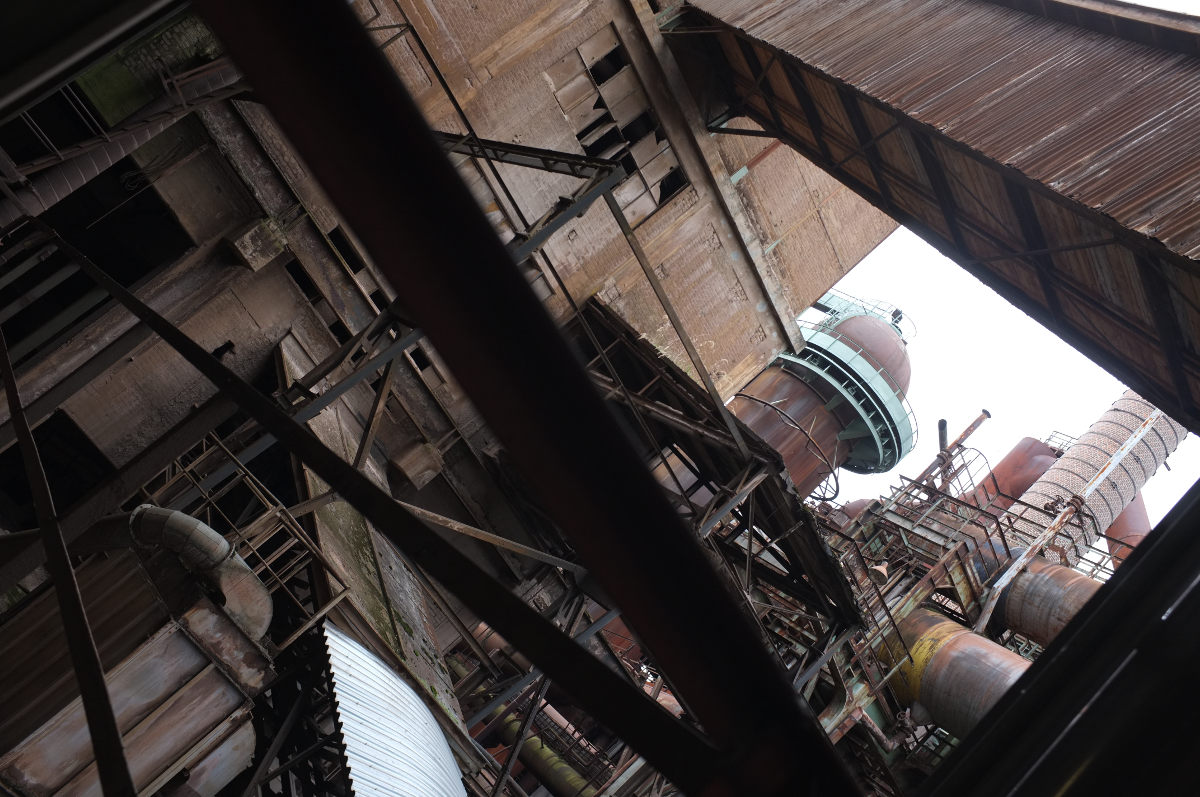
\includegraphics[width=0.7\textwidth]{Examples/example_5.png}
  \caption{Erstes Bild, Völklinger Hütte}
  \label{fig:Huette}
\end{figure}


\subsection{Wrapfigure}
Abbildung~\ref{fig:Huette} ist zwar ganz nett anzusehen, aber vielleicht sähe es eleganter aus, wenn die Abbildung 
von unserem Textabschnitt umflossen werden würde. Diese Art von Abbildungen sollte jedoch sparsam und mit großer Sorgfalt eingesetzt werden, da es zu unschönen Darstellungen kommen kann.
\blindtext
\begin{wrapfigure}{l}{0.4\textwidth}
  \centering
  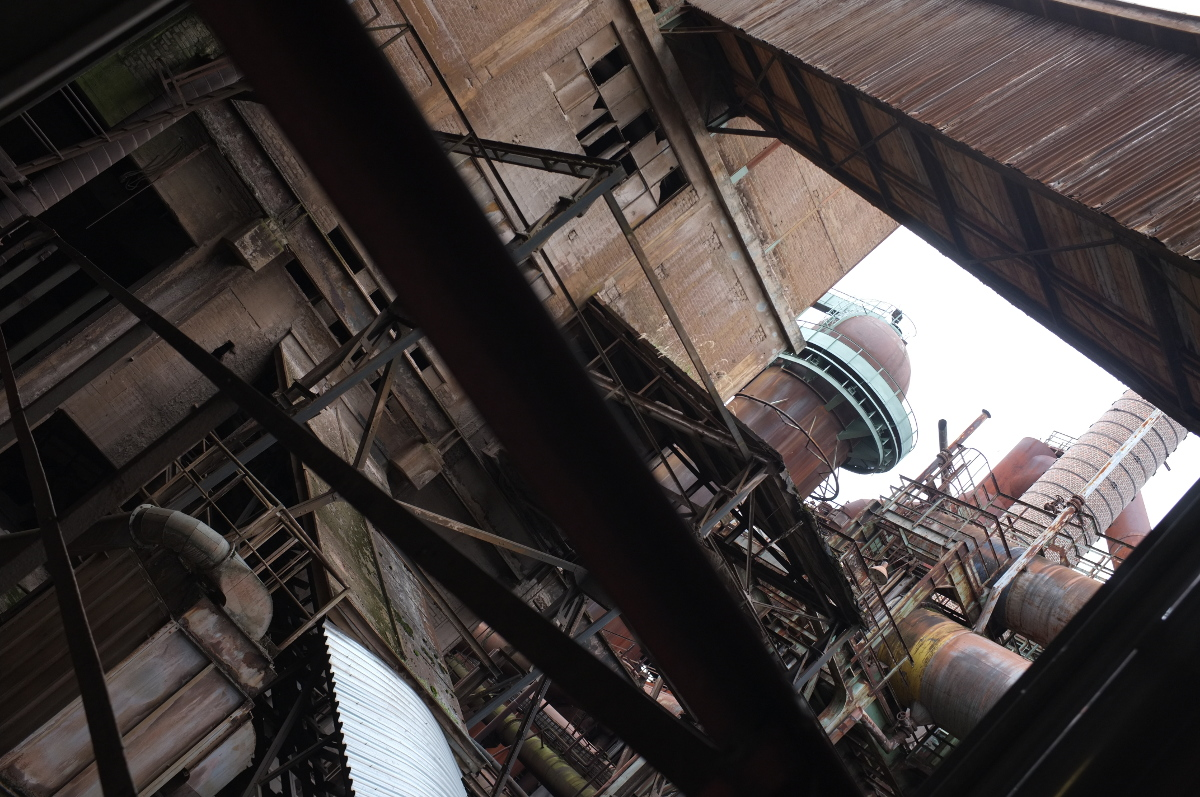
\includegraphics[width=0.4\textwidth]{Examples/example_5.jpg}
  \caption{Völklinger Hütte, *.jpg}
  \label{fig:Huette2}
\end{wrapfigure}
\blindtext


\subsection{Subfigures}
Es ist ebenso möglich, mehrere Abbildungen nebeneinander zu setzen, wie in Abbildung~\ref{fig:Beide} zu sehen ist. Eine separate Referenzierung ist auch möglich: Abbildung~\ref{subfig:abbone}.
\begin{figure}[bth]
  \subfloat[Erstes ...]{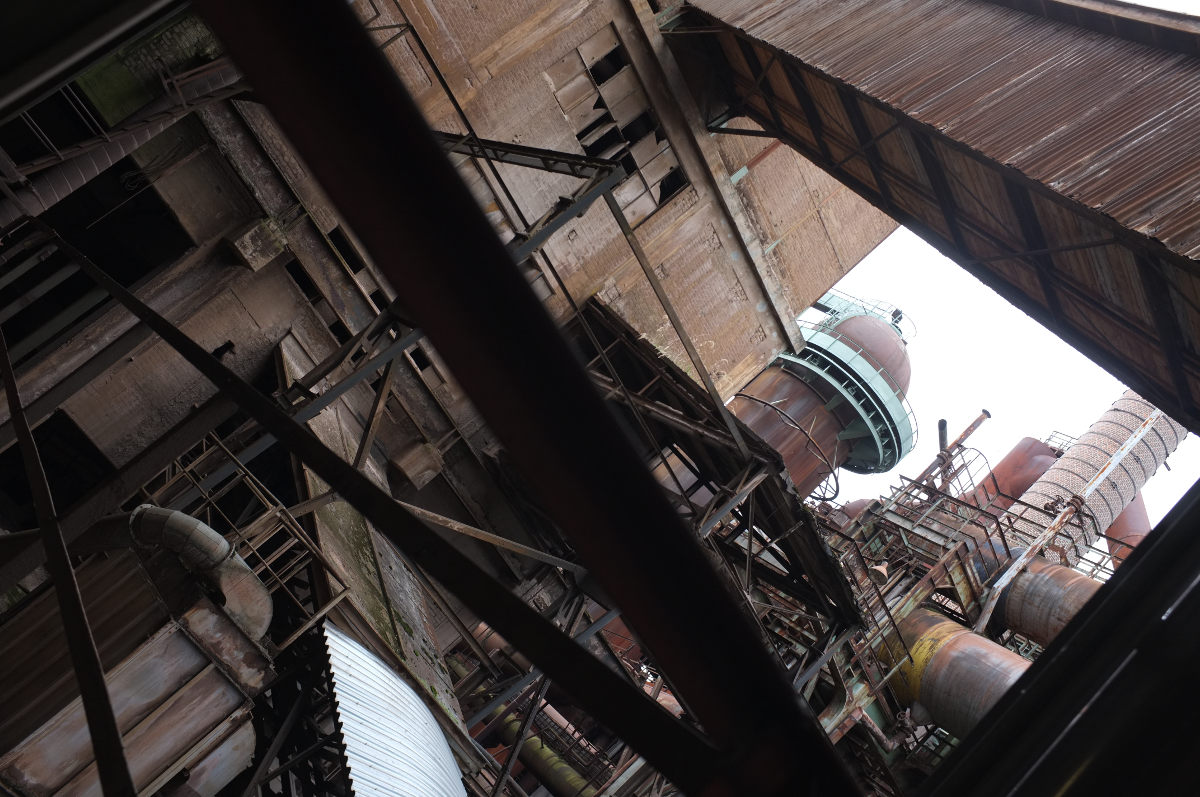
\includegraphics[width=0.49\textwidth]{Examples/example_5.png}\label{subfig:abbone}}\hfill
  \subfloat[... und zweites Bild]{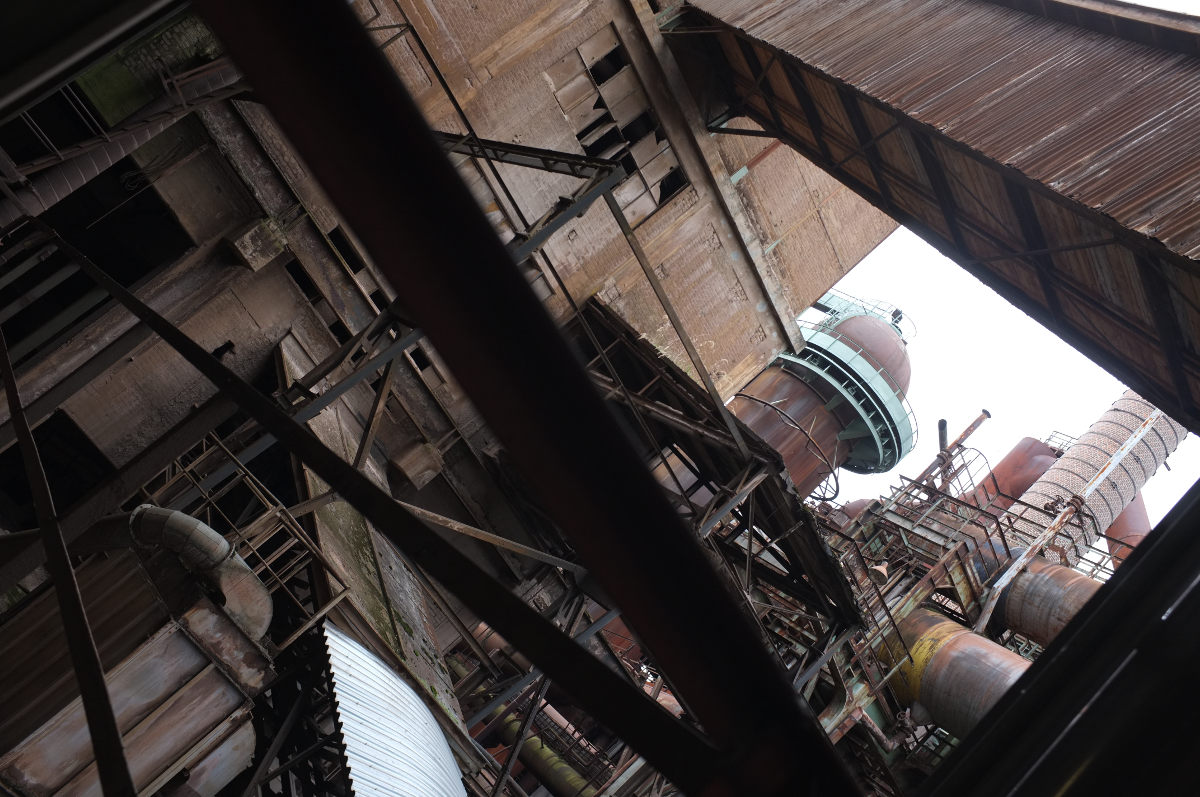
\includegraphics[width=0.49\textwidth]{Examples/example_5.png}\label{subfig:abbtwo}}
  \caption{Mehrere Abbildungen nebeneinander}
  \label{fig:Beide}
\end{figure}


\subsection{Qualitätsunterschiede}
\begin{figure}[p]
	\centering
  \subfloat[\textit{PDF}-Format]{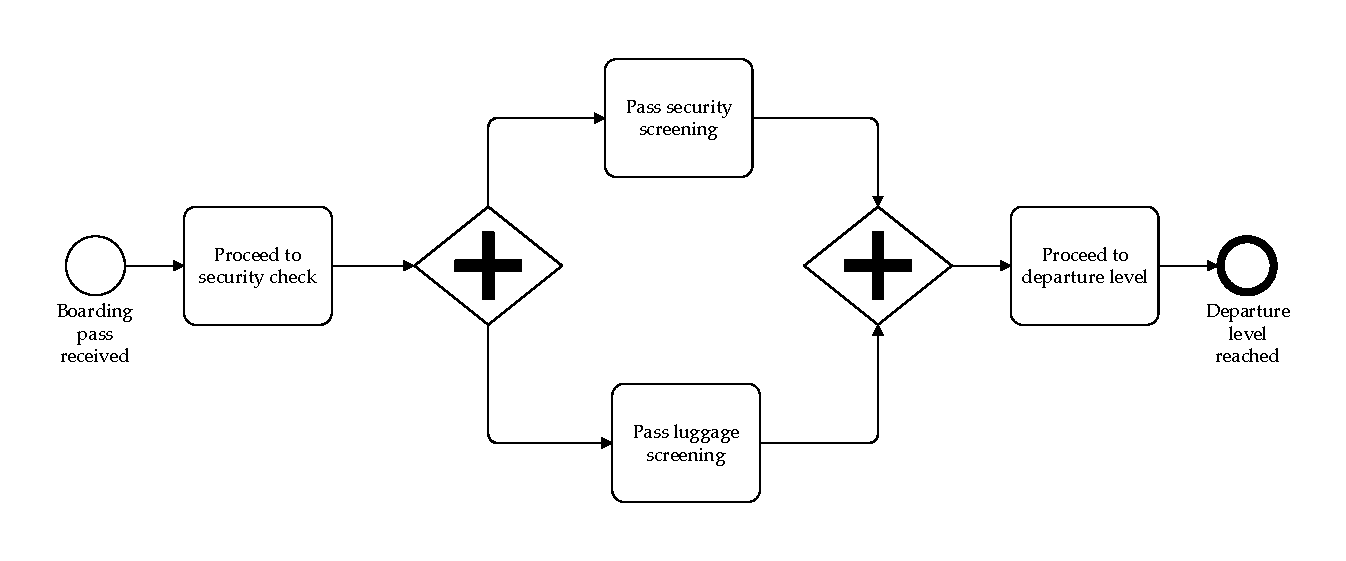
\includegraphics[width=0.65\textwidth]{Examples/bpmn.pdf}} \\
  \subfloat[\textit{JPG}-Format]{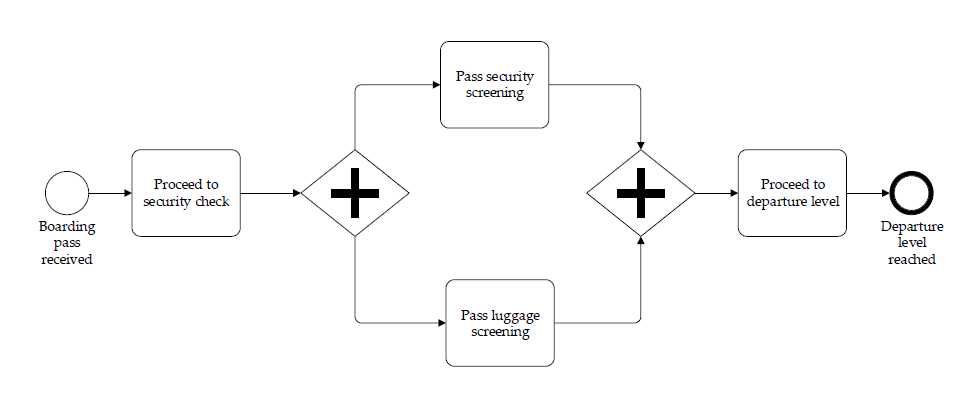
\includegraphics[width=0.65\textwidth]{Examples/bpmn.jpg}}
  \caption{Beide Formate im Vergleich}
  \label{fig:pdfvsjpg}
\end{figure}

\begin{figure}[p]
	\centering
  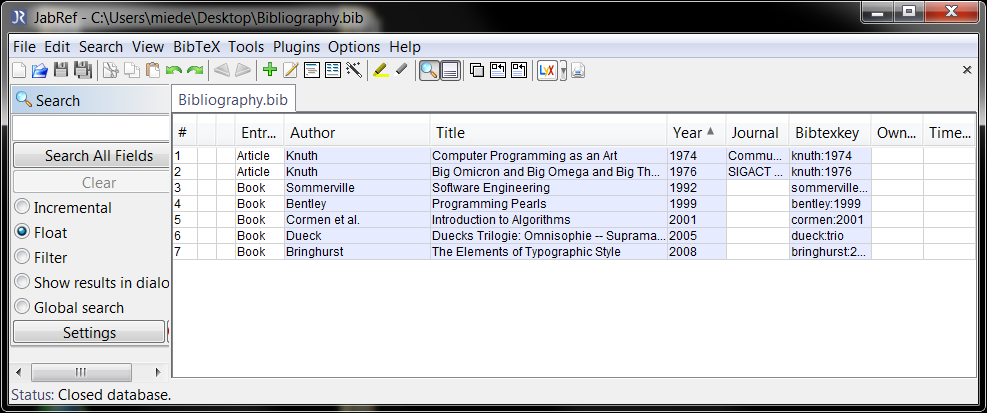
\includegraphics[width=0.65\textwidth]{Examples/jabref.png}
   \caption{\textit{PNG}-Format}
  \label{fig:pngvsjpg1}
\end{figure}

\begin{figure}[p]
	\centering
  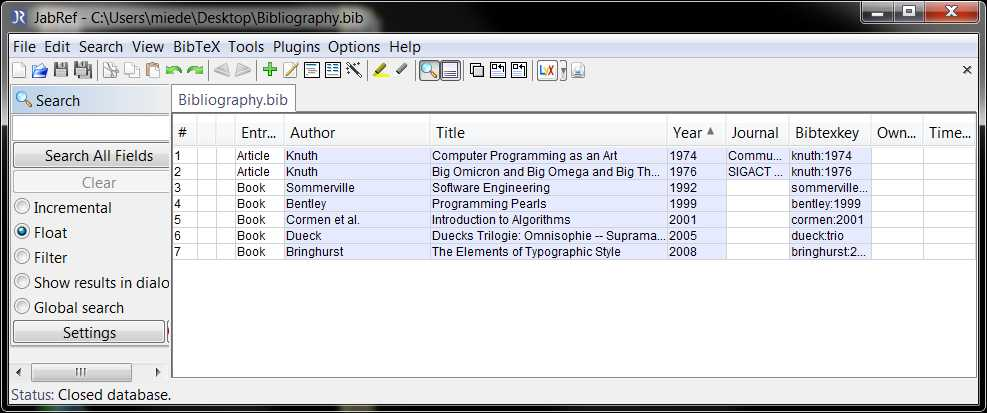
\includegraphics[width=0.65\textwidth]{Examples/jabref.jpg}
   \caption{\textit{JPG}-Format}
  \label{fig:pngvsjpg2}
\end{figure}

Leider haben die unterschiedlichen Grafikformate bedingt durch die unterschiedlichen Kompressionsverfahren einige Schwächen, insbesondere die Umwandlung in das \textit{JPG}-Format erzeugt unangenehme Artefakte im Bild. \autoref{fig:pdfvsjpg} zeigt die Unterschiede zwischen \textit{PDF-Format} und \textit{JPG-Format} im Vergleich. 

Wenn eine \textit{*.pdf}-Datei nicht infrage kommt, beispielsweise bei Screenshots, ist unbedingt das \textit{PNG-Format} vorzuziehen. 
Den Unterschied machen \autoref{fig:pngvsjpg1} und \autoref{fig:pngvsjpg2} deutlich.

"`Faustregeln"' im Umgang mit Abbildungen:
\begin{itemize}
	\item Diagramme bzw. alles, was Linien usw. enthält: \textit{PDF} (im Vektorformat).
	\item Screenshots bzw. alles, was größere gleichfarbige Flächen enthält: \textit{PNG}.
	\item Der Rest (in der Regel Fotos): \textit{JPEG}.
\end{itemize}





%*******************************
% 			Listings 		   *
%*******************************

\section{Quellcode einbinden}
Das Package \textit{lstlisting} ermöglicht es, Quellcode ansprechend in das Dokument einzubinden. Man kann Quellcode einzeilig einbinden 
mittels \lstinline{\lstinline|Quellcode|}. Dabei ist darauf zu achten, dass der Befehl einmal mit \{ \} und einmal mit | | aufgerufen werden kann, je nachdem, 
welche Zeichen im angegebenen Quelltext genutzt werden. 
Es ist auch möglich eine eigene Umgebung für Quelltext zu schaffen:

\begin{lstlisting}[caption=Erstes Listing,style=Java]
private Umgebung(int i, int k)
{
	System.out.println("Eine Funktion mit " + i + "und" + k ".");
}
\end{lstlisting}  

Wer Quelltext aus externen Dateien einbinden möchte, geht wie folgt vor:

\lstinputlisting
[caption={Externer Quellcode},style=Java]
{Examples/Code.java}

Wie genau der Quellcode formatiert und gefärbt ist, ist in \textit{htwsaar.i.mst.config.tex} hinterlegt, wobei fü verschiedene Sprachen auch eigene Styles angelegt werden
können (hier z.B. für Java).
\section{Mathematische Ausdrücke}
Mathematische Ausdrücke sind eine kleine Kunst für sich. Am allereinfachsten kann man eine Formel, wie \(a + b = c\) in den Fließtext einbinden, wobei LaTeX die Höhe der Ausdrücke der Zeile anpasst,
wie hier zu sehen \(\sum_{y=0}^{x} a\) . In einer Umgebung sieht das schon anders aus:
\begin{equation}
  \sum_{y=0}^{x} a
\end{equation}

Griechische Buchstaben:
\begin{equation}
	\alpha\beta\gamma\delta\epsilon\varepsilon\zeta\eta
	\theta\iota\kappa\lambda\mu\nu\xi\pi\varpi\rho\varrho
	\sigma\tau\upsilon\phi\varphi\chi\psi\omega
\end{equation}

Brüche:
\begin{equation}
	Ergebnis = \frac{a}{b}
\end{equation}

\begin{equation}
	\frac{\sin{\alpha}^2 + \cos{\alpha}^2}{1} = 1
\end{equation}

\begin{equation}
	\frac{-9x}{\frac{2y}{3z+2}}
\end{equation}

Text innerhalb von Formeln:
\begin{equation}
\sum_{y=1}^{n} y = \frac{n*(n+1)}{2}
\quad
\text{Gaußsche Summenformel}
\end{equation}

Hoch- bzw. Tiefstellungen:
\begin{equation}
	x_{i,j}^2
\end{equation}

\begin{equation}
	{x_{i,j}}^2
\end{equation}

\begin{equation}
	x_{n_0}
\end{equation}


Matrizen:
Matrizen werden innerhalb der mathematischen Umgebung als wiederum neue Umgebung eingebunden. Wie bei Tabellen auch werden Zeilen durch \lstinline{\\} und Spalten durch \lstinline{&} getrennt.

\begin{equation}
	\begin{pmatrix} 
		a&b\\
		c&d 
	\end{pmatrix}
\end{equation} 

\begin{equation}
	\begin{vmatrix} 
		a&b\\
		c&d 
	\end{vmatrix}
\end{equation} 

Fallunterscheidung:
\begin{equation}
	f(x) = 
	\begin{cases}
		0, &\text{falls } x < 0 \\
		1, &\text{falls } x \geq 0
	\end{cases}
\end{equation}




%############################################################
\clearpage\section{To-Do-Notes}
Um bei einer längeren Arbeit nicht den Überblick zu verlieren, an welcher Stelle es nötig ist
weiter zu arbeiten, bietet es sich an, kleine Notizen einzufügen. Das Package \textit{todonotes}
stellt eine elegante Lösung bereit, um differenziert und vielfarbig jene Abschnitte zu kennzeichnen,
die einer weiteren Bearbeitung bedürfen.

\subsection*{Beispiel für To-Do-Notes}
Dies hier ist ein Blindtext zum Testen von Textausgaben. Wer diesen Text liest, ist selbst
\todo{Plain todonotes.} schuld. Der Text gibt lediglich den Grauwert der Schrift an. Ist das wirklich so? Ist es
gleichgültig, ob ich schreibe: Dies ist ein Blindtext? oder Huardest gefburn? Kjift?
mitnichten! Ein Blindtext bietet mir wichtige Informationen. An ihm messe ich die Les-
barkeit einer Schrift, ihre Anmutung, \todo{Plain todonotes.}wie harmonisch die Figuren zueinander stehen
und prüfe, wie breit oder schmal sie läuft. Ein Blindtext sollte möglichst viele verschie-
dene Buchstaben enthalten und in der Originalsprache gesetzt sein. Er muss keinen
Sinn ergeben, sollte aber lesbar sein.\todo[nolist]{Todonote that is only shown in the margin and not in
the list of todos.}%
Fremdsprachige Texte wie Lorem ipsum dienen
nicht dem eigentlichen Zweck, da sie eine falsche Anmutung vermitteln. Dies hier ist
ein Blindtext zum Testen von Textausgaben. Wer diesen Text liest, ist selbst schuld. 

\todo[inline]{A very long todonote that certainly will fill more
than a single line in the list of todos. Just to make sure let's add
some more text \ldots}

Der Text gibt lediglich den Grauwert der Schrift an. Ist das wirklich so? Ist es gleichgültig,
ob ich schreibe: Dies ist ein Blindtext? oder Huardest gefburn? Kjift? mitnichten!
\todo[noline]{A note with no line back to the text.}
Ein Blindtext bietet mir wichtige Informationen. An ihm messe ich die Lesbarkeit einer
Schrift, ihre Anmutung, wie harmonisch die Figuren zueinander stehen und prüfe, wie
\todo[caption={A short entry in the list of todos}]{A very long
todonote that certainly will fill more than a single line in the
list of todos \ldots}
breit oder schmal sie läuft. Ein Blindtext sollte möglichst viele verschiedene Buchstaben
enthalten und in der Originalsprache gesetzt sein. Er muss keinen Sinn ergeben, sollte
aber lesbar sein. Fremdsprachige Texte wie Lorem ipsum dienen nicht dem eigentlichen Zweck, 
da sie eine falsche Anmutung vermitteln.
\missingfigure{A figure I have to make \ldots}

%Nummerierte ToDo-Notes
\todox{Erste Nummer...}
\todox{Zweite Nummer...}

%Alles To-Dos als Liste ausgegeben
Nachfolgend wird noch eine Liste aller To-Dos auf einer separaten 
Seite ausgegeben.
%\begingroup
	%\let\clearpage\relax
	%\let\cleardoublepage\relax
	\listoftodos
%\endgroup 



%********************************************************************
% Bibliography/References
%*******************************************************
\cleardoublepage%********************************************************************
% Bibliography
%*******************************************************
\printbibliography

%********************************************************************
% List of Figures etc.
%*******************************************************
\cleardoublepage%*******************************************************
% Verzeichnisse (Abbildungen, Tabellen, Listings, etc.)
%*******************************************************
\cleardoublepage
\begingroup
	\let\clearpage\relax
	\let\cleardoublepage\relax
	\listoffigures
	\listoftables
	%\addcontentsline{toc}{chapter}{\lstlistlistingname}
	\lstlistoflistings 
\endgroup 
%*******************************************************
% Abkürzungsverzeichnis
%*******************************************************
\chapter*{Abkürzungsverzeichnis}
\markboth{Abkürzungsverzeichnis}{}
\addcontentsline{toc}{chapter}{Abkürzungsverzeichnis}	
	%Hier alle benötigten Abkürzungen einfügen
	\begin{acronym}[BBPE] % LONGEST ACRONYM HERE FOR CORRECT SPACING
	    \acro{API}{Programmierschnittstelle}
	    \acro{BBPE}{Byte-Level Byte-Pair Encoding}
	    \acro{BCI}{Brain-Computer-Interface}
	    \acro{CPU}{Hauptprozessor}
	    \acro{CSV}{Comma-Separated Values}
	    \acro{EEG}{Elektro\-enzephalo\-graphie}
	    \acro{FFT}{Fast Fourier Transform}
	    \acro{GPU}{Grafikprozessor}
	    \acro{ID}{Identifikationsnummer}
	    \acro{LLM}{Large Language Model}
	    \acro{LoRA}{Low-Rank Adaptation}
	    \acro{OOM}{Out of Memory}
	    \acro{PSS}{Proportional Set Size}
	    \acro{RAM}{Arbeitsspeicher}
	    \acro{SNR}{Signal-Rausch-Verhältnis}
	    \acro{TTFT}{Zeit bis zum ersten Token}
	\end{acronym}
	
	

% ********************************************************************
% Appendix/Anhang
%***************************************************************
\appendix
\part*{Anhang}
\cleardoublepage%********************************************************************
% Appendix
%*******************************************************
\chapter{Aufbereitete Feature-Texte der Evaluation}
\label{app:featuretexte}
Die folgenden Feature-Texte wurden vom \texttt{FeatureFormatter} aus den beiden Sessions erzeugt und den Modellen als Eingabe übergeben (vgl.\ \autoref{subsec:eval-beispiele}). Sie ermöglichen es, die Modellausgaben gegen die tatsächliche Eingabe zu prüfen.

\begin{figure}[H]
\centering
{\setlength{\fboxsep}{12pt}\fcolorbox{blue!30}{blue!5}{%
\begin{minipage}{0.9\linewidth}
\sffamily\small
EEG-Session, Dauer 121.432s, 8 Kanäle.\\[5pt]
Abschnitt 1 (0.0--30.352s):\\
\hspace*{1.5em}Delta 86\%, Theta 4\%, Alpha 5\%, Beta 3\%, Gamma 2\%\\
\hspace*{1.5em}Ungültige Messwerte: 0.0\% ungültig, größter Ausschlag Kanal 4 (4419 µV)\\[5pt]
Abschnitt 2 (30.356--60.708s):\\
\hspace*{1.5em}Delta 59\%, Theta 16\%, Alpha 13\%, Beta 7\%, Gamma 5\%\\
\hspace*{1.5em}Ungültige Messwerte: 0.0\% ungültig, größter Ausschlag Kanal 2 (3309 µV)\\[5pt]
Abschnitt 3 (60.712--91.064s):\\
\hspace*{1.5em}Delta 56\%, Theta 18\%, Alpha 13\%, Beta 7\%, Gamma 6\%\\
\hspace*{1.5em}Ungültige Messwerte: 0.0\% ungültig, größter Ausschlag Kanal 2 (2874 µV)\\[5pt]
Abschnitt 4 (91.068--121.432s):\\
\hspace*{1.5em}Delta 63\%, Theta 11\%, Alpha 11\%, Beta 8\%, Gamma 8\%\\
\hspace*{1.5em}Ungültige Messwerte: 0.0\% ungültig, größter Ausschlag Kanal 2 (2948 µV)
\end{minipage}}}
\caption{Feature-Text der Session A (Grundlage für Report und Artefakt-Erklärung).}
\label{fig:ft-session-a}
\end{figure}

\begin{figure}[H]
\centering
{\setlength{\fboxsep}{12pt}\fcolorbox{blue!30}{blue!5}{%
\begin{minipage}{0.9\linewidth}
\sffamily\small
EEG-Session, Dauer 122.128s, 8 Kanäle.\\[5pt]
Abschnitt 1 (0.0--30.528s):\\
\hspace*{1.5em}Delta 86\%, Theta 5\%, Alpha 3\%, Beta 4\%, Gamma 2\%\\
\hspace*{1.5em}Ungültige Messwerte: 0.0\% ungültig, größter Ausschlag Kanal 2 (5230 µV)\\[5pt]
Abschnitt 2 (30.532--61.06s):\\
\hspace*{1.5em}Delta 77\%, Theta 9\%, Alpha 6\%, Beta 5\%, Gamma 3\%\\
\hspace*{1.5em}Ungültige Messwerte: 0.0\% ungültig, größter Ausschlag Kanal 2 (4772 µV)\\[5pt]
Abschnitt 3 (61.064--91.592s):\\
\hspace*{1.5em}Delta 73\%, Theta 10\%, Alpha 6\%, Beta 7\%, Gamma 4\%\\
\hspace*{1.5em}Ungültige Messwerte: 0.0\% ungültig, größter Ausschlag Kanal 2 (3878 µV)\\[5pt]
Abschnitt 4 (91.596--122.128s):\\
\hspace*{1.5em}Delta 66\%, Theta 15\%, Alpha 8\%, Beta 6\%, Gamma 5\%\\
\hspace*{1.5em}Ungültige Messwerte: 0.0\% ungültig, größter Ausschlag Kanal 2 (3518 µV)
\end{minipage}}}
\caption{Feature-Text der Session B (zweite Session im Vergleich).}
\label{fig:ft-session-b}
\end{figure}


%*******************************************************
\cleardoublepage\pagestyle{empty}

\hfill

\vfill


\pdfbookmark[0]{Kolophon}{colophon}
\section*{Kolophon}
Dieses Dokument wurde mit der \LaTeX-Vorlage für Abschlussarbeiten an der htw saar im Bereich Informatik/Mechatronik-Sensortechnik erstellt (\currentVersion). Die Vorlage wurde von Yves Hary und Andr\'e Miede entwickelt (mit freundlicher Unterstützung von Thomas Kretschmer, Helmut G. Folz und Martina Lehser). Daten: (F)\makeatletter\f@size\makeatother\ -- (B)\the\textwidth\ -- (H)\the\textheight\ 


\end{document}
% ********************************************************************
